\chapter{Learning and Generalisation}
\section{Probably Approximately Correct (PAC) Learning: Terms}
\begin{enumerate}
    \item A is impossible: $P(A) = 0$
    \item A is certain: $P(A) = 1$
    \item A is almost certain: $P(A) \approx 1$
    \item A is probable: $(P(A) > 0) \wedge (P(A) < 1)$
    \item A is correct if error $\varepsilon_A = 0$
    \item A is approximately correct: $\varepsilon_A \approx 0$, very small
    \item A is probably (how certain?) correct: $P(\varepsilon_A = 0) \approx 1$
    \item A is probably approximately correct (P.A.C.): $P(\varepsilon_A > B)$ with $B \approx 1$
\end{enumerate}

\section{Hoeffding's Inequality}

Hoeffding's Inequality is a foundational result in probability theory and statistics, especially within machine learning and statistical learning theory. It offers bounds on the probability that the sample mean of independent and identically distributed (i.i.d.) random variables deviates from its expected value.

\begin{sidenotebox}{Statement of Hoeffding's Inequality (General Case)}

For a sequence of independent and bounded random variables $X_1, X_2, \ldots, X_n$, each lying in the range $a \leq X_i \leq b$, the sample mean $\bar{X}$ adheres to the following inequality:

\begin{equation}
P\left(\left|\bar{X} - \mu\right| \geq \epsilon\right) \leq 2\exp\left(-\frac{2n\epsilon^2}{(b - a)^2}\right)
\end{equation}

Where:
\begin{itemize}   
\item  $\bar{X}$ represents the sample mean.
\item  $\mu$ denotes the true expected value of $X_i$.
\item  $a$ and $b$ are the respective lower and upper bounds of $X_i$.
\item  $\epsilon$ indicates the deviation from the expected value.
\item  $n$ is the sample count.
\end{itemize}
\end{sidenotebox}


\begin{sidenotebox}{Derivation of Hoeffding's Inequality for Binary Classification}
Note to self: proof from https://nowak.ece.wisc.edu/SLT07/lecture7.pdf is much cleaner and concise. Replace

\subsubsection{Preliminaries}
Given independent random variables \(X_1, X_2, \ldots, X_n\) where each \(i\) satisfies \(a_i \leq X_i \leq b_i\), define \(S_n = \sum_{i=1}^{n} X_i\) and \(E[S_n] = \sum_{i=1}^{n} E[X_i]\).

\subsubsection{Theorem: Chernoff Bound}
For any positive \(t\):
\begin{align*}
\mathbb{P}(S_n - E[S_n] \geq \epsilon) &\leq \mathbb{P}(e^{tS_n} \geq e^{t(E[S_n] + \epsilon)}) \\
&\leq \frac{\mathbb{E}[e^{tS_n}]}{e^{t(E[S_n] + \epsilon)}}
\end{align*}
Given the independence of the \(X_i\)'s:
\begin{align*}
\mathbb{E}[e^{tS_n}] &= \mathbb{E}\left[\exp\left(t\sum_{i=1}^{n} X_i\right)\right] \\
&= \prod_{i=1}^{n} \mathbb{E}[e^{tX_i}]
\end{align*}

\subsubsection{Exponential Moments}
Considering that for \(0 \leq \lambda \leq 1\), \(e^x \leq \lambda e^{\frac{x}{\lambda}} + (1-\lambda)\):
\begin{align*}
\mathbb{E}[e^{tX_i}] &\leq \mathbb{E}\left[\lambda e^{\frac{ta_iX_i}{\lambda}} + (1-\lambda)e^{\frac{tb_iX_i}{1-\lambda}}\right] \\
&= \lambda e^{\frac{ta_i}{\lambda}} + (1-\lambda)e^{\frac{tb_i}{1-\lambda}}
\end{align*}

\subsubsection{Combine and Optimise}
Starting from our earlier result using the Chernoff bound:
\[ \mathbb{P}(S_n - E[S_n] \geq \epsilon) \leq \frac{\mathbb{E}[e^{tS_n}]}{e^{t(E[S_n] + \epsilon)}} \]

And using the exponential moments bound we derived:
\[ \mathbb{E}[e^{tX_i}] \leq \lambda e^{\frac{ta_i}{\lambda}} + (1-\lambda)e^{\frac{tb_i}{1-\lambda}} \]

Substituting in, we get:
\[ \mathbb{E}[e^{tS_n}] \leq \prod_{i=1}^{n} \left( \lambda e^{\frac{ta_i}{\lambda}} + (1-\lambda)e^{\frac{tb_i}{1-\lambda}} \right) \]

The optimization step involves selecting values of \(t\) and \(\lambda\) that minimize the right-hand side of this inequality, given our constraints. For Hoeffding's inequality, in the context of binary classification, where \(a_i = 0\) and \(b_i = 1\), we optimize for this specific case – this step is non-trivial.\\


Substituting the exponential moments into the Chernoff bound and performing optimization over \(t\) and \(\lambda\), we get:
\begin{align*}
\mathbb{P}(S_n - E[S_n] \geq \epsilon) &\leq \exp\left(-\frac{2\epsilon^2}{\sum_{i=1}^{n} (b_i - a_i)^2}\right)\\
\mathbb{P}(\bar{X} - \mu \geq \epsilon) &\leq 2\exp\left(-\frac{2\epsilon^2n}{(b - a)^2}\right)
\end{align*}
To account for both sides of the deviation (positive and negative), we multiply the right-hand side by 2, arriving at the given form of Hoeffding's inequality.
\end{sidenotebox}


\subsection{Hoeffding's Inequality}
Using Hoeffding's inequality, we can then write:

\begin{definitionbox}{Hoeffding's Inequality}
\[
P\left(\left|\widehat{R}_n(h) - R(h)\right| \geq \epsilon\right) \leq 2\exp\left(-2n\epsilon^2\right)
\]

\begin{itemize}
    \item \(\widehat{R}_n(h)\) - The empirical risk or empirical error rate of hypothesis \(h\), which is the average error over a sample of size \(n\). This is our training data.
    \item \(R(h)\) - The true risk or true error rate of hypothesis \(h\), which represents the expected error rate over all possible instances.
    \item \(n\) - The sample size or the number of instances tested against the hypothesis \(h\).
\end{itemize}


\end{definitionbox}

Which provides a bound on the probability that the empirical risk deviates from the true risk by at least \(\epsilon\).

\subsection{Understanding Hoeffding's Inequality through the Dice-Roll example}

Hoeffding's Inequality provides a bound on the probability that the sum of independent, bounded random variables deviates from its expected value. To get an intuitive understanding, let's consider the simple example of rolling a fair six-sided dice.\\


Given a fair six-sided dice, each face has an equal probability of $\frac{1}{6}$ of landing. Thus, the expected value, \( E[X] \), of a single dice roll is:

\[ E[X] = \frac{1}{6}(1) + \frac{1}{6}(2) + \frac{1}{6}(3) + \frac{1}{6}(4) + \frac{1}{6}(5) + \frac{1}{6}(6) = 3.5 \]


Now, let's roll the dice \( n \) times and compute the average, \( \bar{X}_n \), of the rolls. As we roll the dice more and more, we expect \( \bar{X}_n \) to get closer to the expected value, 3.5.

Hoeffding's Inequality states that for any \( \epsilon > 0 \):

\[ P(|\bar{X}_n - E[X]| > \epsilon) \leq 2 \exp\left(-2n\epsilon^2\right) \]

This means the probability that our average deviates from the expected value by more than \( \epsilon \) decreases exponentially as the number of rolls, \( n \), increases. In simpler terms, the more we roll the dice, the closer our average gets to 3.5, and the probability of a significant deviation becomes very small.\\

For instance, if after rolling the dice 1000 times our average is 3.4 or 3.6 (which is \( \epsilon = 0.1 \) away from 3.5), Hoeffding's Inequality gives an upper bound on how likely this event is. And as mentioned, the more rolls we have, the tighter this bound becomes, ensuring our empirical average approaches the true expected value.\\

Hoeffding's Inequality gives us a formal, mathematical guarantee on the convergence of empirical averages to their expected values, as demonstrated with our dice roll example.






\section{Probability vs. Expectation}
For any event, there exists a true probability, denoted by \( P(\text{event}) \), and an expectation, denoted by \( \mathbb{E}[\text{event}] \). While one might anticipate these to be approximately equal, in many cases (e.g., polls), they can significantly differ. \\

We notate the as $p_{\text{event}} = P(\text{event})$ and $e_{\text{event}}$ = $\mathbb{E}[\text{event}]$ \\

One example:\\

Imagine that there is a small town with only 100 voters and two candidates running for mayor: Alice and Bob. A polling company does a survey and finds the following probabilities for voter preference:

\begin{itemize}
    \item 50\% of voters prefer Alice.
    \item 45\% of voters prefer Bob.
    \item 5\% of voters are undecided.
\end{itemize}

If we only consider the probabilities, one might simply conclude that Alice is more likely to win since she has a higher percentage of voter preference.\\

Now, expectation: suppose in reality, the undecided voters are learning towards Bob because of a recent positive news story about him, and 80\% of the undecided voters will go for Bob and 20\% for Alice.\\

For Alice:
\begin{align*}
    \text{Expected votes} &= (\text{Probability of Alice}) \times (\text{Total voters}) \\
    &\quad + (\text{Probability of undecided}) \times (\text{Probability of choosing Alice}) \times (\text{Total voters}) \\
    &= 0.50 \times 100 + 0.05 \times 0.20 \times 100 \\
    &= 50 + 1 \\
    &= 51 \text{ votes}
\end{align*}

For Bob:
\begin{align*}
    \text{Expected votes} &= (\text{Probability of Bob}) \times (\text{Total voters}) \\
    &\quad + (\text{Probability of undecided}) \times (\text{Probability of choosing Bob}) \times (\text{Total voters}) \\
    &= 0.45 \times 100 + 0.05 \times 0.80 \times 100 \\
    &= 45 + 4 \\
    &= 49 \text{ votes}
\end{align*}

Even considering the expected swing from the undecided voters towards Bob, Alice still has a higher expected vote count. However, the gap has narrowed considerably when we take the expected behaviour of undecided voters into account. The initial probabilities alone would not have shown us this nuance.

\begin{commentbox}{Author's Comment on Probability vs Expectation}
In machine learning (or at least, this module), the expectation is used to refer to the ground truth (in our example, this is the actual expected outcomes of the election), which we are trying to approximate with our samples of training data (which is the poll in our example). Our model was not complex enough to account for undecided voters swinging to either Alice or Bob, despite our approximation turning out correct in the end.
\end{commentbox}

\subsection{Hoeffding's Inequality in Learning}
Hoeffding's inequality offers a bound on how the empirical average (or empirical risk) of i.i.d. random variables deviates from its expectation. For any \( \epsilon > 0 \):
\begin{align*}
P(e_{\text{event}} - p_{\text{event}} > \epsilon) & \leq \delta \\
P(e_{\text{event}} - p_{\text{event}} \leq \epsilon) & \leq e^{-2\epsilon^2n} \quad \text{(one-sided)} \\
P(|e_{\text{event}} - p_{\text{event}}| > \epsilon) & \leq 2e^{-2\epsilon^2n} \quad \text{(two-sided)}
\end{align*}

An important implication of Hoeffding's inequality is the concept of being \textit{Probably Approximately Correct (PAC)}. In the realm of machine learning, this means that our empirical estimates are likely close to the true values, but not always exact.\\

\begin{definitionbox}{Empirical and True risk}
In the context of learning, we denote:
\begin{itemize}
    \item \( \widehat{R}_n(h) \): Empirical risk (training error), which is the approximation of the true risk based on our training data set. This is our $p_{\text{event}}$.
    \item \( R(h) \): True risk (test error), which is the expectation of the error over the entire probability distribution of the data. This is the ground truth, which in practice, we do not have access to. This is our $e_{\text{event}}$.
\end{itemize}
    
\end{definitionbox}
With Hoeffding's inequality, we can assert that:
$$
P(|\widehat{R}_n(h) - R(h)| > \epsilon) \leq 2e^{-2\epsilon^2n}
$$
This showcases the closeness of the training error to the test error, given sufficient samples.


\subsection{Assumptions}
One critical assumption for Hoeffding's inequality to hold is that the data samples \( x \) are independent and identically distributed (i.i.d.). This means that each data sample is drawn independently from the same distribution \( P(\mathcal{X}) \). This assumption ensures that the empirical averages are meaningful estimates of the true averages.

\section{Error Measures in Learning}

The core of learning theory revolves around approximating an unknown target function using available data. The degree of approximation is quantified using error measures, also referred to as loss functions.

\subsection{Error Measures or Loss Functions}
Given a hypothesis class \( \mathcal{H} \) and a target function, it is crucial to quantify how well a chosen hypothesis \( h \) approximates the target. Loss functions measure the discrepancy between the predictions made by \( h \) and the actual values:
\begin{itemize}
    \item \textbf{Squared Error}: \( \ell(y, \widehat{y}) = (y - \widehat{y})^2 \)
    \item \textbf{Binary Error}: \( \ell(y, \widehat{y}) = \mathbb{I}(y \neq \widehat{y}) \)
\end{itemize}

\subsection{Training vs. Test Error}
The training error measures the discrepancy on the dataset used to find \( h \), while the test error gives an expectation of the error on new, unseen data:
\begin{align*}
    \text{Training Error:} \quad & R_{\text{in}}(h) = \frac{1}{n} \sum_{i=1}^{n} \ell(h(x_i), y_i) \\
    \text{Test Error:} \quad & R(h) = \mathbb{E}[\ell(h(x), y)]
\end{align*}

$\ell$ is the error function that depends on what type of machine learning methods we are using.

\subsection{Error Costs and Decision Making}
In some scenarios, different types of errors might incur different costs. For instance, in medical diagnosis, a false negative (diagnosing a diseased patient as healthy, for example) might have a more severe consequence than a false positive (diagnosing a healthy patient as diseased). 

\subsection{Error Costs in Machine Learning}
The process of learning in machine learning models involves minimising errors based on certain criteria. Depending on the specific problem and requirements, different error costs can be considered.

\begin{itemize}
    \item \textbf{Equally Penalising Errors:} In some scenarios, all types of errors, be it false positive or false negative, are penalised equally.
    \item \textbf{Aggressively Penalising False Negatives:} In critical scenarios such as medical diagnosis, a false negative (failing to detect a disease when it is present) could have dire consequences, and hence is penalised heavily.
    \item \textbf{Risk Aversion by Penalising False Positives:} In other situations, such as spam email detection, false positives (classifying legitimate email as spam) might be more costly.
\end{itemize}

\subsection{Binary Error and the Indicator Function}\label{indicatorfunc}
The binary error, which checks if the predicted output matches the actual output, uses the indicator function. The function is defined as:
\[
\mathbb{I}(a \neq b) = 
\begin{cases} 
1 & \text{if } a \neq b \\
0 & \text{otherwise}
\end{cases}
\]
In the context of learning, the binary error is used to check if the hypothesis $h(x)$ is equal to the true function value $f(x)$. If they are not equal, the error is 1, otherwise it is 0.

\begin{table}[H]
\centering
\begin{tabular}{|c|c|c|}
\hline
& $f = +1$ & $f = -1$ \\
\hline
$h = +1$ & No error & False positive \\
\hline
$h = -1$ & False negative & No error \\
\hline
\end{tabular}
\caption{Two types of error}
\end{table}

The two primary types of errors are:
\begin{itemize}
    \item \textbf{False Negative (Type I error)}: The model rejects a scenario when it should have accepted it.
    \item \textbf{False Positive (Type II error)}: The model accepts a scenario when it should have rejected it.
\end{itemize}

\subsection{Penalizing Errors}

\begin{table}[H]
\centering
\begin{tabular}{|c|c|c|}
\hline
& $f = +1$ & $f = -1$ \\
\hline
$h = +1$ & 0 & 1 \\
\hline
$h = -1$ & 1 & 0 \\
\hline
\end{tabular}
\caption{Equally penalizing errors}
\end{table}

\begin{table}[H]
\centering
\begin{tabular}{|c|c|c|}
\hline
& $f = +1$ & $f = -1$ \\
\hline
$h = +1$ & 0 & 100 \\
\hline
$h = -1$ & 1 & 0 \\
\hline
\end{tabular}
\caption{Risk averse: false positive is expensive}
\end{table}

\begin{table}[H]
\centering
\begin{tabular}{|c|c|c|}
\hline
& $f = +1$ & $f = -1$ \\
\hline
$h = +1$ & 0 & 1 \\
\hline
$h = -1$ & 100 & 0 \\
\hline
\end{tabular}
\caption{Aggressive: false negative is expensive}
\end{table}



Different penalties can be assigned to each type of error based on the requirements of the specific application. For example, in scenarios like medical diagnosis, a false negative might be heavily penalised.

\begin{commentbox}{Author's Comment on Semantics of `Risk Averse' and `Aggressive'}
    Note that this module uses `risk averse' to discourage false positives and `aggressive' to discourage false negatives, in practice this terminology can vary. It is more precise to describe models based on their preference for minimising one type of error over the other, or for being balanced in treating both types of errors.
\end{commentbox}



\section{Probabilistic Learning Framework}
\subsection{Considering Noise, Learning with Noisy Data (Stochastic Noise)}\label{learning_with_noise}
\begin{commentbox}{Note to Reader: Module Arrangement}
    The module notes defines the grounds for probabilistic learning here, but does not elaborate further until the next chapter where we apply these concepts.
\end{commentbox}


Machine learning, in practice, often faces the challenge of having to deal with inherent uncertainties present in real-world data, in the form of noise. \\

Instead of a deterministic output \( y = f(x) \), the relationship may be probabilistic \( y \sim P(y|x) \), allowing for the same input to yield different outputs.\\

Data points \( (x, y) \) are generated from a joint distribution \( P(x, y) \), which can be decomposed as:

$$ P(x,y) = P(y|x)P(x) $$


We model noise in the data as 

$$ y = f(x) + N $$

where $N$ is noise, $f(x) = \mathbb{E}[y|x]$  and $\mathbb{E}[N|x] = 0$. \\

An example would be $y=w^\top x + N$ where $N \sim \mathcal{N}(0, \Sigma)$ is independent of $x$. \\

In the special case of the deterministic problem, there is zero noise $N= 0$ and $P(y|x)$ is concentrated on the single form f(x).

\subsection{Errors and the Learning Setup}

To make the most accurate predictions, the choice of an optimal hypothesis function \( h \) is influenced by both the nature of noise in the data and the form of the loss function used to measure prediction errors.

\begin{itemize}
    \item \textbf{Squared Error Loss:} When using squared error loss, denoted by \( \ell(y, \widehat{y}) = (y - \widehat{y})^2 \), the optimal decision rule \( g(x) \) is the one that minimises the expected squared error, $\mathbb{E}[(y-h(x))^2|x]$ across the data distribution. Formally, it is the expected value of the target variable given the input, \( g(x) = \mathbb{E}[y|x] \).
    
    \item \textbf{Binary Error Loss:} For classification tasks where the error is binary, expressed as \( \ell(y, \widehat{y}) = \mathbb{I}(y \neq \widehat{y}) \) where \( \mathbb{I} \) is the indicator function, the optimal hypothesis \( g(x) \) is that which maximizes the probability of the correct label being chosen. In mathematical terms, \( g(x) \) is the class that has the maximum posterior probability given the input, \( g(x) = \underset{y}{\arg\max}\, P(y|x) \).
\end{itemize}

This subsection emphasises the reliance of the optimal decision on the choice of the loss function, whether it is for regression with squared error or for classification with binary error, taking into account the statistical properties of the data.


We aim to develop a model to make accurate predictions or decisions based on input data amidst noise. This process involves selecting an appropriate hypothesis from a set of potential candidates. 

\begin{definitionbox}{Learning Setup Overview}
    

\begin{itemize}
    \item \textbf{Input and Output:} The learning algorithm receives an input \( x \in \mathcal{X} \) and predicts an output \( y \in \mathcal{Y} \). The true relationship between inputs and outputs is governed by the unknown probability distribution \( P(y|x) \), which the learning algorithm tries to approximate.
    $$ \{(x_1, y_1), (x_2, y_2), \ldots, (x_n, y_n)\}  \sim P$$
    
    \item \textbf{Data:} We collect a dataset \( \{(x_1, y_1), (x_2, y_2), \ldots, (x_n, y_n)\} \) which is assumed to be sampled from the joint distribution \( P(x, y) \). This dataset serves as the empirical basis for learning the input-output mapping.
    
    \item \textbf{Hypothesis Class:} The hypothesis class \( \mathcal{H} \) is the set of all functions \( h: \mathcal{X} \rightarrow \mathcal{Y} \) that the learning algorithm considers. The choice of \( \mathcal{H} \) can significantly impact the algorithm's ability to generalise from the training data to unseen data.
    $$
    \mathcal{H} \subset \{h:\mathcal{X} \rightarrow \mathcal{Y}\}
    $$
    
    \item \textbf{Loss Function:} The loss function \( \ell: \mathcal{Y} \times \mathcal{Y} \rightarrow \mathbb{R} \) quantifies how far off a prediction is from the actual value. It provides a criterion for evaluating the quality of a hypothesis.
    
    \item \textbf{Learning Objective:} The goal of learning is to find a hypothesis \( g \in \mathcal{H} \) that best approximates the true distribution \( P(y|x) \). Formally, we seek a hypothesis that minimises the expected loss over the data distribution: 
    $$ g = \arg\min_{h \in \mathcal{H}} \mathbb{E}[\ell(h(x), y)] $$
    
    \item \textbf{Aggregation Strategy:} While the expectation is a common way to aggregate the loss over the distribution, alternative strategies may be required in certain situations, such as when the distribution \( P \) is highly imbalanced. This consideration is crucial for ensuring that the model performs well across all segments of the data, not just the majority class.
\end{itemize}

\end{definitionbox}

The process of choosing \( \mathcal{H} \) is non-trivial and depends on several factors, including the complexity of the data, the type of problem (regression or classification), and the computational resources available. This choice determines the hypothesis space within which our optimal model will be found and, consequently, the success of our learning algorithm in making accurate predictions.\\

For a fixed single hypothesis $h \in \mathcal{H}$, the learning process uses the familiar Hoeffding's Inequality:

\begin{itemize}
    \item \textbf{Training Error (Empirical Risk):} The training error is the average loss over the training set, and it is denoted by \( \widehat{R}_n(h) \). For a training set of size \( n \), it is defined as:
    \[
    \widehat{R}_n(h) = \frac{1}{n} \sum_{i=1}^{n} \ell(h(x_i), y_i);
    \]
    where \( \ell \) is the loss function, \( h(x_i) \) is the prediction of hypothesis \( h \) for input \( x_i \), and \( y_i \) is the true output.

    \item \textbf{Test Error (Out-of-Sample Risk):} The test error is the expectation of the loss function over the joint distribution of inputs and outputs. It is denoted by \( R(h) \) and represents the true risk of hypothesis \( h \). It can be expressed in two ways:
    \begin{itemize}
        \item \( R(h) = \mathbb{P}(h(x_i) \neq f(x_i)); \)
        \item \( R(h) = \mathbb{E}[\widehat{R}_n(h)]; \)
    \end{itemize}
    where \( f \) is the true function that we are trying to approximate. The test error is a measure of how well the hypothesis generalises to new data that were not seen during training.
\end{itemize}

Again as usual, by Hoeffding's Inequality:
\[
P\left(\left|\widehat{R}_n(h) - R(h)\right| \geq \epsilon\right) \leq 2\exp\left(-2n\epsilon^2\right)
\]

The discrepancy between training error and test error relates the concept of overfitting, where a hypothesis may perform well on the training data but poorly on new data due to its failure to generalise.




\subsection{Generalisation for Multiple Hypotheses}
When working with a hypothesis class \( \mathcal{H} \), we are often interested in the performance of not just one, but all hypotheses within this class, so we can choose the best model from the class set. To extend Hoeffding's inequality to the entire class, we employ the union bound. This approach provides a way to aggregate the probabilities of multiple independent events, extending the Hoeffding's inequality to handle multiple hypotheses.\\

     Let \( \mathcal{H} = \{h_1, h_2, \ldots, h_M\} \) be a finite hypothesis class with \( M \) distinct hypotheses. The probability that at least one hypothesis \( h \in \mathcal{H} \) has a large deviation between its empirical risk \( \widehat{R}_n(h) \) and true risk \( R(h) \) is given by the union bound:

    \[P\left( \bigcup_{m=1}^{M} \{ |\widehat{R}_n(h_m) - R(h_m)| > \varepsilon \} \right) = 
    P\left( \max_{h \in \mathcal{H}} |\widehat{R}_n(h) - R(h)| > \varepsilon \right) \leq \sum_{m=1}^{M} P\left( |\widehat{R}_n(h_m) - R(h_m)| > \varepsilon \right).
    \]

    Using Hoeffding's inequality for each hypothesis, we have:

    \[
    P\left( |\widehat{R}_n(h_m) - R(h_m)| > \varepsilon \right) \leq 2e^{-2n\varepsilon^2},
    \]

    which gives us the union bound for all \( M \) hypotheses:

    \begin{equation}
    P\left( \max_{h \in \mathcal{H}} |\widehat{R}_n(h) - R(h)| > \varepsilon \right) \leq 2Me^{-2n\varepsilon^2}.
    \label{eq:union_bound}
    \end{equation}

    \begin{commentbox}{Why take the union bound?}
        The union bound is taken as a worst-case scenario approach to probability. When dealing with multiple hypotheses, we want to ensure that our bound on the generalisation error holds not just for a single hypothesis but for all hypotheses in our class.\\

        In the context of machine learning, each hypothesis could potentially overfit the training data and not generalise well to new, unseen data. The union bound helps us assess this risk across all hypotheses by combining their individual risks. This way, we can make a statement like "with high probability, none of the hypotheses will have a generalisation error greater than some specified bound," giving us confidence that the hypothesis we select from this class will perform well on new data.
    \end{commentbox}

     To understand the square root and logarithm in the derived bound, we define \( \delta \) such that \( \delta = 2Me^{-2n\varepsilon^2} \), leading to \( \varepsilon = \sqrt{\frac{1}{2n}\log\frac{2M}{\delta}} \). This rearrangement comes from solving the equation for \( \varepsilon \) in terms of \( \delta \) and \( M \) (the number of hypotheses). \\


\begin{definitionbox}{Multiple Hypotheses Generalisation Bound}    
     Thus, with probability at least \( 1 - \delta \), for all hypotheses \( h \in \mathcal{H} \) simultaneously, we have:
    \[
    |\widehat{R}_n(h) - R(h)| \leq \sqrt{\frac{1}{2n}\log\frac{2M}{\delta}}
    \]
\begin{itemize}
    \item \( \widehat{R}_n(h) \) is the empirical risk of the hypothesis \( h \), calculated from the training data.
    \item \( R(h) \) is the true risk of the hypothesis \( h \), considering the entire data distribution.
    \item \( M \) represents the size of the hypothesis class \( \mathcal{H} \)
    \item \( \delta \) is a parameter that controls the confidence level of the bound: with probability at least \( 1 - \delta \), the bound holds.
    \item \( n \) is the size of the training data.
\end{itemize}

This inequality is a statement about the uniform convergence of the empirical risk to the true risk for all hypotheses in the class.\\

More specifically, it shows, that with high probability, the true risk of any hypothesis in the class will not deviate from the empirical risk observed on the training data by more than the bound on the RHS.\\

The RHS probabilistic bound $ \sqrt{\frac{1}{2n}\log\frac{2M}{\delta}}$ is the difference between empirical risk and true risk for any hypothesis within the hypothesis class.\\

This also means that if we minimise empirical risk, we are likely to be close to minimising true risk, which is our goal.


\end{definitionbox}



\subsection{Empirical Risk Minimisation (ERM)}

Empirical Risk Minimisation (ERM) is a principle used to select a hypothesis from a hypothesis class \( \mathcal{H} \) based on empirical (test) data. Let us denote the optimal hypothesis in \( \mathcal{H} \) by \( h^* \), which is the hypothesis that minimises the true risk \( R(h) \):

\begin{equation*}
    h^* = \arg\min_{h\in\mathcal{H}} R(h).
\end{equation*}

The aim of ERM is to choose a hypothesis \( g \) from \( \mathcal{H} \) that has the smallest empirical error:

\begin{equation*}
    g = \arg\min_{h\in\mathcal{H}} \widehat{R}_n(h),
\end{equation*}

where \( \widehat{R}_n(h) \) is the empirical risk calculated from the training data.\\

Note that we don't know what is hypothesis $h^*$ because we cannot practically measure true risk $R(h^*)$ (we don't have infinite data samples). But we can calculate empirical risk $\widehat{R}_n{h}$ and therefore identify hypothesis $g$. \\




With the empirical risk minimiser \( g \), we wish to understand how well it approximates the optimal hypothesis \( h^* \) in terms of the true risk. The following bound provides this guarantee:


\begin{definitionbox}{Risk of the Empirical Risk Minimiser}
With probability at least \( 1 - \delta \),

\begin{equation*}
    R(g) - R(h^*) \leq \sqrt{\frac{2 \log \frac{2M}{\delta}}{n}},
\end{equation*}

where \( M \) is the size of the hypothesis class \( \mathcal{H} \), and \( n \) is the size of the sample.\\

Note that the absolute value is no longer needed because $R(g) - R(h^*)$ is always positive, since we assume $h^*$ is the best hypothesis and has the lowest error. Also, note that we are taking the difference in true risk.

\begin{itemize}
    \item Hypothesis \( h^* \) is the optimal hypothesis that has the smallest true risk \( R_n(h^*) \) for the entire data distribution.
    \item Hypothesis \( g \) is the hypothesis we can identify and choose, that has the smallest empirical risk \( \widehat{R}_n(g) \) for our training data.
\end{itemize}

\end{definitionbox}


\textbf{The principle of ERM suggests a practical way to approximate the best possible prediction rule (hypothesis) within the hypothesis class $\mathcal{H}$, based on observed data. \\}

To understand this relationship, the size of this class, denoted by \( M \), directly affects how well the model generalises. A larger \( \mathcal{H} \) implies a more complex model space, which, while potentially leading to a lower empirical risk, can also increase the risk of overfitting. \\

From equation \ref{eq:union_bound}:

\begin{align}
P\left( \max_{h \in \mathcal{H}} |\widehat{R}_n(h) - R(h)| > \varepsilon \right) \leq 2Me^{-2n\varepsilon^2} \label{eq:extension_hoeff_M} \\
P\left(|\widehat{R}_n(g)-R(g)|>\varepsilon\right)\leq 2|\mathcal{H}|e^{-2\varepsilon^2n}
\end{align}


We want a hypothesis that fits the training data well (minimising empirical risk) but also generalise to new, unseen data (minimising true risk).
The complexity of $\mathcal{H}$, quantified by its cardinality \( |\mathcal{H}| \), affects the likelihood of the empirical risk mirroring the true risk.\\


For any fixed hypothesis \( h \in \mathcal{H} \), the probability that the empirical risk deviates from the true risk by more than an amount \( \varepsilon \) is bounded by \( 2e^{-2n\varepsilon^2} \), which reassures us about the stability of the hypothesis:

\[
P\left(|\widehat{R}_n(h)-R(h)|>\varepsilon\right)\leqslant2e^{-2\varepsilon^2n}
\]

However, when we consider a hypothesis \( g \) that has been chosen based on the data (such as one that minimises the empirical risk), we need to account for the selection process from within the hypothesis class. Here, the bound adjusts to include the size of the class, reflecting the added uncertainty from this selection:

\[
P\left(|\widehat{R}_n(g)-R(g)|>\varepsilon\right)\leqslant2|\mathcal{H}|e^{-2\varepsilon^2n}
\]

So we can conclude that $g$ cannot deviate too far from $h^*$, using the data we have.

% \subsection{Choosing the hypothesis}

% The bounds and guarantees discussed provide a foundation for understanding the role of the hypothesis class in the learning process.accurate and robust against overfitting. These theoretical insights are crucial for practical machine learning, where the ultimate goal is to achieve reliable predictions on real-world, unseen data.


% \subsection{Choosing our Hypothesis: Linear Classification Example}


% \subsubsection*{Feature Representation}
% In linear classification, we typically represent features as vectors:
% \begin{equation*}
%     \mathbf{x} = (x_1, \ldots, x_d) \in \mathbb{R}^d
% \end{equation*}
% where \( x_0 = 1 \) is often included to account for the bias term, thus extending the vector into \( \mathbb{R}^{d+1} \).

% \subsubsection*{Labels and Data Points}
% The labels are denoted by \( y \) and can take on values in the set \( \{+1, -1\} \), corresponding to the two classes. We consider \( n \) data points:
% \begin{equation*}
%     (\mathbf{x}_1, y_1), \ldots, (\mathbf{x}_n, y_n),
% \end{equation*}
% where each \( \mathbf{x}_i \) is a feature vector and \( y_i \) is its associated label.

% \subsubsection*{Hypothesis Class}
% The hypothesis class consists of functions parameterised by weight vectors \( \mathbf{w} \):
% \begin{equation*}
%     h_{\mathbf{w}}(\mathbf{x}) = \text{sign}(\mathbf{w}^{\top}\mathbf{x}),
% \end{equation*}
% where \( \mathbf{w} = (w_0, w_1, \ldots, w_d) \) and the sign function returns +1 or -1 depending on the sign of its argument.

% \subsubsection*{The Perceptron Algorithm}
% The perceptron algorithm seeks a hypothesis \( h \in \mathcal{H} \) such that \( h(\mathbf{x}_i) = y_i \) for all \( i = 1, \ldots, n \), assuming such a hypothesis exists within the hypothesis class. The empirical risk minimizer under this setting is:
% $$
%     g = \arg\min_{h \in \mathcal{H}} \sum_{i=1}^{n} \mathbb{I}(h(\mathbf{x}_i) \neq y_i),
% $$
% which corresponds to minimising the number of misclassifications. See \ref{indicatorfunc} for more information on the indicator function $\mathbb{I}$.

\subsubsection*{Applicability of ERM Theory}
When considering ERM in the context of linear classification, a critical question arises: Is the hypothesis class \( \mathcal{H} \) finite? \\

In theory, there are infinite amount of possible weights, as they can take on any real-valued numbers. This is clearly not computable with our current setup – The finiteness of \( \mathcal{H} \) is important for the guarantees of ERM to hold, otherwise the bounds will not be useful (infinitely large $|\mathcal{H}|$ on the RHS of the bound does not give us confidence that the LHS error will be bounded.). In later sections we learn to find a more practical quantity for the number of hypotheses.\\



\section{Growth Function, Shattering, and Break Points}
\subsection{Overlapping Hypotheses Example}\label{overlap_hypo}

\begin{figure}[ht]
    \centering
    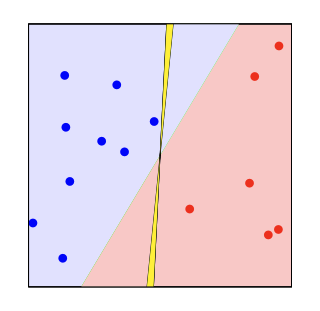
\includegraphics[width=0.4\textwidth]{img/h-overlap.png}
    \caption{Hypotheses that split the points similarly}
    \label{fig:h-overlap}
\end{figure}

In practical machine learning applications, especially in classification problems, we sometimes encounter the situation where two different hypotheses \( h_1 \) and \( h_2 \) provide similar predictions over the training set. This is referred to as overlapping hypotheses. Mathematically, if \( h_1 \approx h_2 \) then it follows that:

\begin{equation*}
    \widehat{R}_n(h_1) \approx \widehat{R}_n(h_2) \quad \text{and} \quad R(h_1) \approx R(h_2),
\end{equation*}

where \( \widehat{R}_n(h) \) represents the empirical risk and \( R(h) \) represents the true risk of a hypothesis \( h \). This indicates that when the hypotheses are similar, their empirical and true risks are expected to be close to each other. Thus:

\begin{equation*}
    |\widehat{R}_n(h_1) - R(h_1)| \approx |\widehat{R}_n(h_2) - R(h_2)|,
\end{equation*}

which implies that a large difference in empirical risk between \( h_1 \) and \( h_2 \) can often indicate a similarly large difference in their true risks. This is an important concept for understanding the performance of learning algorithms. However, it is important to realise that \( h_1 \neq h_2 \) if there exists some \( \textbf{x} \in \mathcal{X} \) where $\mathcal{X}$ is the input space, such that \( h_1(\textbf{x}) \neq h_2(\textbf{x}) \); this is what creates a dichotomy, or a configuration of dividing points, in the hypothesis space.

\[
\left|\widehat{R}_n(h_1) - R(h_1)\right| > \varepsilon \text{ often implies } \left|\widehat{R}_n(h_2) - R(h_2)\right| > \varepsilon
\]

\[
h_1 \neq h_2 \text{ if } \exists \textbf{x} \in \mathcal{X} : h_1(\textbf{x}) \neq h_2(\textbf{x}) \rightarrow \text{ dichotomy}
\]

This is why we only considered a finite sample of $\textbf{x}$ from the input space $\mathcal{X}$ – more than one hypothesis could represent the same dichotomy for a finite amount of points.  


\subsection{Growth Function and Perceptron}

In this section we consider the perspective of including a finite sample of data, $\textbf{x}$ from the input space $\mathcal{X}$.\\

We propose the growth function, a function which quantifies the capacity of a hypothesis class \( \mathcal{H} \) to fit data. It is a function of the number of points \( n \) and is denoted as \( m_{\mathcal{H}}(n) \). This function counts the maximum number of dichotomies—or distinct classifications—of \( n \) points that the hypothesis class can realise. For the perceptron, which is a linear classifier, this function is closely related to the concept of `shattering`.

\begin{definitionbox}{Growth Function}\label{growth_func}
The growth function measures the number maximum number of dichotomies that a hypothesis class can produce on any set of $n$ points from the input space. Intuitively, it tells us how many ways the hypothesis class can label $n$ points, regardless of their actual arrangement in the input space.\\

The growth function for a hypothesis class \( \mathcal{H} \), denoted by \( m_{\mathcal{H}}(n) \), represents the maximum number of dichotomies that can be realised by the hypotheses in \( \mathcal{H} \) on any set of \( n \) points. For a perceptron, this is bounded by the number of hypotheses, and can be formalised as:

\begin{equation*}
    m_{\mathcal{H}}(n) = \max_{\textbf{x}_1,\ldots,\textbf{x}_n \in \mathcal{X}} |\mathcal{H}(\textbf{x}_1, \ldots, \textbf{x}_n)| \leq 2^n,
\end{equation*}

where \( \mathcal{H}(\textbf{x}_1, \ldots, \textbf{x}_n) \) denotes the set of all possible dichotomies on \( n \) points. However, not all sets of points can be shattered by a perceptron, especially if the data is not linearly separable. \\

Note that the upper bound for the growth function is $2^n$ – the maximum number of ways $n$ points can be classed positively or negatively. 
\end{definitionbox}

\begin{definitionbox}{Dichotomies in Machine Learning}
    A dichotomy refers to a particular way of splitting or labelling a set of points into two categories, typically represented as positive (+1) and negative (-1) classes. Dichotomies are used to describe the different possible classifications that a set of data points can have according to the hypotheses within the class.
\end{definitionbox}


\subsection{Shattering and break points}



\begin{definitionbox}{What does it mean to `shatter' (in the context of the perceptron)?}
A set of points is considered to be `shattered` by the hypothesis class \( \mathcal{H} \) if, for every possible binary labelling of these points, there exists a hypothesis in \( \mathcal{H} \) that can produce exactly these labels. The `break point` is the smallest number of points that the hypothesis class cannot shatter, signifying a limit to the complexity of \( \mathcal{H} \).
\end{definitionbox}

\begin{definitionbox}{The Break Point}
    The break point is the smallest number \( k \) such that no set of \( k \) points can be shattered by the hypothesis class \( \mathcal{H} \). For a perceptron, the break point provides insight into the complexity and capacity of the model.\\

    \textbf{Break Point} (capacity of \(\mathcal{H}\)): There exists \( k \) such that \( m_{\mathcal{H}}(k) < 2^k \) which is the size of the largest set \( \{x_1, \ldots, x_k\} \) in \(\mathcal{X}\) that can be shattered by \(\mathcal{H}\).

    \[\exists k:m_{\mathcal{H}(k)}\nexists(\mathbf{x_1},\ldots,\mathbf{x_k})\in\mathcal{X}:\text{shattered by }\mathcal{H})\]

\end{definitionbox}

% \begin{figure}[H]
%     \centering
%     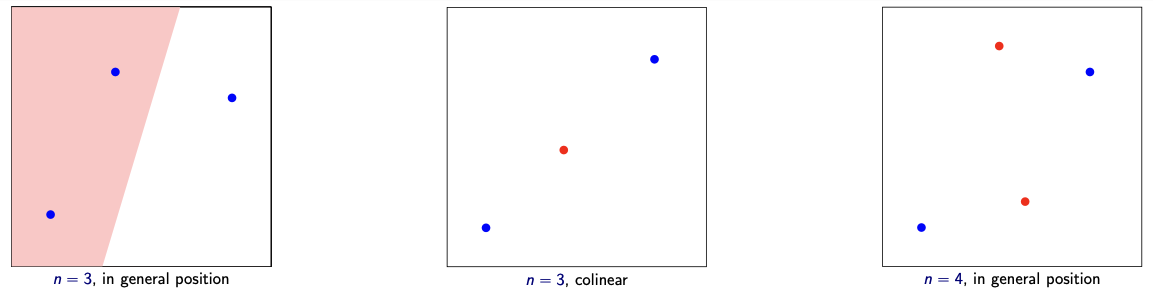
\includegraphics[width=1\textwidth]{img/shatter-dich.png}
%     \caption{2D perceptron shattering configurations}
%     \label{fig:shatter-dich}
% \end{figure}
\begin{figure}[h!]
    \centering
    \begin{subfigure}[b]{0.2\textwidth}
        \centering
        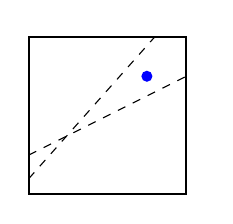
\begin{tikzpicture}
            \draw[thick] (-1,-1) rectangle (1,1);
            \fill[blue] (0.5,0.5) circle (2pt);
            \draw[dashed] (-1,-0.5)--(1,0.5) node[right] {};
            \draw[dashed] (-1,-0.8)--(0.6,1) node[right] {};
        \end{tikzpicture}
        \caption{Shattering 1 point}
    \end{subfigure}
    \hfill
    \begin{subfigure}[b]{0.2\textwidth}
        \centering
        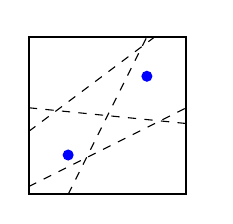
\begin{tikzpicture}
            \draw[thick] (-1,-1) rectangle (1,1);
            \fill[blue] (-0.5,-0.5) circle (2pt);
            \fill[blue] (0.5,0.5) circle (2pt);
            \draw[dashed] (-1,0.1)--(1,-0.1) node[right] {};
            \draw[dashed] (-1,-0.9)--(1,0.1) node[right] {};
            \draw[dashed] (-1,-0.2)--(0.6,1) node[right] {};
            \draw[dashed] (-0.5,-1)--(0.5,1) node[right] {};
        \end{tikzpicture}
        \caption{Shattering 2 points}
    \end{subfigure}
    \hfill
    \begin{subfigure}[b]{0.2\textwidth}
        \centering
        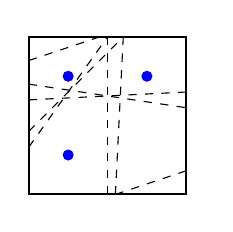
\begin{tikzpicture}
            \draw[thick] (-1,-1) rectangle (1,1);
            \fill[blue] (0.5,0.5) circle (2pt);
            \fill[blue] (-0.5,0.5) circle (2pt);
            \fill[blue] (-0.5,-0.5) circle (2pt);
            \draw[dashed] (-1,-0.4)--(0,1) node[right] {};
            \draw[dashed] (-1,-0.2)--(0.2,1) node[right] {};
            \draw[dashed] (-1,0.2)--(1,0.3) node[right] {};
            \draw[dashed] (-1,0.4)--(1,0.1) node[right] {};
            \draw[dashed] (0,1)--(0,-1) node[right] {};
            \draw[dashed] (0.2,1)--(0.1, -1) node[right] {};
            \draw[dashed] (1,-0.7)--(0.1, -1) node[right] {};
            \draw[dashed] (-1,0.7)--(-0.1,1) node[right] {};
        \end{tikzpicture}
        \caption{Shattering 3 points}
    \end{subfigure}
    \hfill
    \begin{subfigure}[b]{0.2\textwidth}
        \centering
        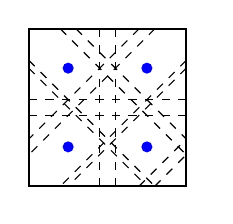
\begin{tikzpicture}
            \draw[thick] (-1,-1) rectangle (1,1);
            \fill[blue] (0.5,0.5) circle (2pt);
            \fill[blue] (0.5,-0.5) circle (2pt);
            \fill[blue] (-0.5,0.5) circle (2pt);
            \fill[blue] (-0.5,-0.5) circle (2pt);
            \draw[dashed] (-1,0.1)--(1,0.1) node[right] {};
            \draw[dashed] (-1,-0.1)--(1,-0.1) node[right] {};
            \draw[dashed] (0.1,1)--(0.1,-1) node[right] {};
            \draw[dashed] (-0.1,1)--(-0.1,-1) node[right] {};
            \draw[dashed] (0.4,1)--(-1,-0.4) node[right] {};
            \draw[dashed] (0.6,1)--(-1,-0.6) node[right] {};
            \draw[dashed] (1,0.6)--(-0.6,-1) node[right] {};
            \draw[dashed] (1,0.5)--(-0.5,-1) node[right] {};

            \draw[dashed] (-0.4,1)--(1,-0.4) node[right] {};
            \draw[dashed] (-0.6,1)--(1,-0.6) node[right] {};
            \draw[dashed] (-1,0.6)--(0.6,-1) node[right] {};
            \draw[dashed] (-1,0.5)--(0.5,-1) node[right] {};

            
            
            


            \draw[dashed] (0.4,-1)--(1,-0.4) node[right] {};
            \draw[dashed] (0.6,-1)--(1,-0.6) node[right] {};
            

        \end{tikzpicture}
        \caption{Shattering 4 points}
    \end{subfigure}
    \caption{Perceptron shattering points on a 2D plane.}
    \label{fig:2d_perceptron}
\end{figure}

\begin{itemize}
    \item Given a 2D perceptron and a single point, the single point can be classified as +1 or -1. The total number of dichotomies, $m_\mathcal{H}(1)$, is 2. The 2D perceptron can shatter a single point.
    \item Given a 2D perceptron and two points, either both points are +1 or -1, or they are one of each. There are 4 dichotomies, $m_\mathcal{H}(2)= 4$. The 2D perceptron can shatter two points.
    \item A 2D perceptron can fully shatter a maximum of 3 points, unless they are collinear, in which case some separations are not possible. Still, the maximum number of dichotomies are 8, $m_\mathcal{H}(2)= 8$
    \item Once you have four points, they can be geometrically considered as the vertices of a convex quadilateral. Labelling opposite vertices with the same class show that no single line can separate the classes. So four points cannot be shattered, so 4 is the break point for a 2D perceptron. Still, there are 14 possible dichotomies, $m_\mathcal{H}(4)=14  $
\end{itemize}

A 2D perceptron can fully shatter a maximum of 3 points, unless they are collinear, in which case some separations are not possible.\\

We then introduce the notion of the Combinatorial Quantity function:
\subsection{The Combinatorial Quantity \( B(N, k) \)}\label{combinatorial_quantity}

\begin{commentbox}{Note to Self: Notation check}
    Is $B(N,k)$ referring to the combinatorial quantity for a perceptron, or is it general? Please fix notation soon
\end{commentbox}

This is a measure of how many dichotomies can you list on \( N \) points so that no \( k \) are shattered. $k$ is the break point, defined in the previous section. Intuitively, it is the list of all possible combinations, `$N$ choose $i$', or $\textbf{C}_i^N$, for values of $i$ up to $k-1$.

\[ B(N, k): \text{Max. number of dichotomies on } N \text{ points so that no } k \text{ are shattered.} \]

\begin{table}[h!]
\centering
\begin{tabular}{|c|c|c|}
\hline
\( X_1 \) & \( X_2 \) & \( X_3 \) \\
\hline
\Circle   & \Circle   & \Circle   \\
\Circle   & \Circle   & \CIRCLE   \\
\Circle   & \CIRCLE   & \Circle   \\
\CIRCLE   & \Circle   & \Circle   \\
\CIRCLE   & \CIRCLE   & \Circle   \\
\Circle   & \CIRCLE   & \CIRCLE      \\
\CIRCLE   & \Circle   & \CIRCLE      \\
\hline
\end{tabular}
\quad
\begin{tabular}{|c|c|c|c|}
\hline
\( X_1 \) & \( X_2 \) & \( X_3 \) &\( X_4 \) \\
\hline
\Circle & \Circle & \Circle & \Circle \\
\Circle & \Circle & \Circle & \CIRCLE \\
\Circle & \Circle & \CIRCLE & \Circle \\
\Circle & \CIRCLE & \Circle & \Circle \\
\CIRCLE & \Circle & \Circle & \Circle \\
\hline
\end{tabular}
\caption{Visualisation of dichotomies for \( B(3,3) \) and \( B(4,2) \). \(B(3,3) = 5, B(4,2) = 5 \)}
\end{table}

It is easy to see that \[ B(N, k) \leq \sum_{i=0}^{k-1} \binom{N}{i} . \]
Note we use the inequality for the combinatorial quantity function – an easy example why we do this is because not every hypothesis class can achieve every combination. For example, in Figure \ref{fig:2d_perceptron}, for the 2D perceptron with four points and break point 4, there are only 14 possible dichotomies. If we enumerated the general case using our visualisation in \ref{combinatorial_quantity}, we could get up to $\textbf{C}^4_3+\textbf{C}^4_2+\textbf{C}^4_1+\textbf{C}^4_0 = 15$, which is greater than 14.

\begin{sidenotebox}{Bound of Combinatorial Quantity Function}\label{combquant_function_bound}
\textbf{Theorem (actually a form of the Sauer-Shelah Lemma)}
\[ B(N, k) \leq \sum_{i=0}^{k-1} \binom{N}{i} . \]

\textbf{Proof Sketch}
(Induction on \(N\).)
\begin{enumerate}
    \item Verify for \(N = 1\): \( B(1,1) \leq 1 \) \checkmark
    \item Suppose \( B(N, k) \leq \sum_{i=0}^{k-1} \binom{N}{i} \).
\end{enumerate}

\textbf{Lemma (Pascal's Identity)}
\[ \binom{N}{k} + \binom{N}{k-1} = \binom{N+1}{k} . \]

    



Then,
\begin{align*}
B(N + 1, k) &\leq B(N, k) + B(N, k - 1) \\
&\leq \sum_{i=0}^{k-1} \binom{N}{i} + \sum_{i=0}^{k-2} \binom{N}{i} \\
&= 1 + \sum_{i=1}^{k-1} \left( \binom{N}{i} + \binom{N}{i-1} \right) \quad (\text{by lemma}) \\
&= 1 + \sum_{i=1}^{k-1} \binom{N+1}{i} \\
&= \sum_{i=0}^{k-1} \binom{N+1}{i}
\end{align*}

A clearer explanation of the recurrence relation can be watched \href{https://youtu.be/6FWRijsmLtE?si=Tg2jX1YDYAjXFdE0&t=372}{here}, courtesy of the Caltech ML Lectures. \\

\textbf{To show the bound is polynomial in k:}
\[ B(N, k) \leq \sum_{i=0}^{k-1} \binom{N}{i} . \]
\begin{align*}
    \sum_{i=0}^{k-1} \binom{N}{i} \leq \left(\frac{N}{k-1}\right)^{k-1} \sum_{i=0}^{k-1} \binom{k-1}{i} \left(\frac{k-1}{N}\right)^i\\
\leq \left(\frac{N}{k-1}\right)^{k-1} \sum_{i=0}^{k-1} \binom{k-1}{i} \left(\frac{k-1}{N}\right)^m\\
\leq \left(\frac{N}{k-1}\right)^{k-1} \left(1 + \frac{k-1}{N}\right)^m\\
\leq \left(\frac{N}{k-1}\right)^{k-1} e^{k-1} \\
\end{align*}


\end{sidenotebox}

We show the combinatorial quantity \( B(N, k) \) is polynomial. So for the perceptron and any other ML methods that have a finite break point, the growth function $m_\mathcal{H}$  is polynomial as well.  \\

Also, we realise that $B(N,k)$ is actually the general growth function that tells you the total number of possible dichotomies for a given number of data points $N$ and break point k. The growth function $m_\mathcal{H}(n)$ tells you the total number of possible dichotomies for a hypothesis $\mathcal{H}$ that has a pre-determined constant $k$ that we don't have to show, for $n$ points.\\

From Hoeffding's Inequality in \ref{eq:extension_hoeff_M}:

\begin{align*}
P\left( \max_{h \in \mathcal{H}} |\widehat{R}_n(h) - R(h)| > \varepsilon \right) \leq 2Me^{-2n\varepsilon^2} 
=_{\text{somewhat, but not quite}}P\left( \sup_{h \in \mathcal{H}} |\widehat{R}_n(h) - R(h)| > \varepsilon \right) \leq 2m_{\mathcal{H}}(n)e^{-2n\varepsilon^2}
\end{align*}

Here, we've tried replacing the count of hypotheses $M$ with the growth function, $m_{\mathcal{H}}(n)$, which bounds the numbers of ways $\mathcal{H}$ can label any set of $n$ points.
This step is motivated by the realisation that not all hypotheses in $\mathcal{H}$ are distinct when considering how they label a finite set of points – many hypotheses might make the same predictions, so the true ``size" of $\mathcal{H}$ with respect to the dataset is better captured by $m_{\mathcal{H}}(n)$ than $M$. \\

Note that what we did was merely to illustrate our understanding, but we actually cannot simply interchange $M$ with the growth function. Through a lot more technicality and change of constants, we can produce the Vapnik-Chervonenkis inequality which is sound. This is covered further in the Caltech lectures \href{https://youtu.be/6FWRijsmLtE?si=fP-5cgJ52UhqAIGI&t=3484}{here}.\\


Earlier in \ref{growth_func}, we could define the growth function $m_{\mathcal{H}}$ having an upper bound of $2^n$.\\

This is unfortunately not low enough, because having an exponential $n$ within the bound will interfere with the $e^{-2n\epsilon^2}$ part for large $n$, and we cannot be sure that the difference between empirical and true error will be bounded.\\

However, since we can show that $m_{\mathcal{H}}$ is polynomial, we have no problems with the right-hand-side bound because the $e^{-2n\epsilon^2}$ part overrules the $m_{\mathcal{H}}(n)$.

\begin{itemize}
    \item If there is no break point, the growth function \( m_{\mathcal{H}}(n) \) is equal to \( 2^n \), which is the maximum number of dichotomies possible for binary classification on \( n \) points.
    \item If a break point \( k \) exists, \( m_{\mathcal{H}}(k) \) is polynomial in \( n \), indicating that the number of dichotomies is less than the maximum, thus reflecting a constraint in the hypothesis class. This is because $\mathcal{O}(2^n) > \mathcal{O}(n^k)$.
    \item Such a polynomial is expressed as \( m_{\mathcal{H}}(k) = a_kn^k + a_{k-1}n^{k-1} + \ldots + a_1n + a_0 \), where the coefficients \( a_i \) correspond to the complexity of dichotomies at different levels.

\end{itemize}

The notes stop short of a detailed proof for going from Hoeffding's inequality to the Vapnik-Chernovenkis inequality, yet they present us with an equation that, while not entirely precise, serves as an illustrative stepping stone toward understanding the Vapnik-Chernovenkis Inequality.




\subsection{The Vapnik-Chervonenkis Inequality}\label{vc-ineq-subsection}



We can consider the VC-dimension, which is a measure of the capacity or complexity of a classification algorithm. More specifically, the VC-dimension, denoted as \( d_{VC}(\mathcal{H}) \), measures the capacity of \( \mathcal{H} \) by the size of the largest set of points that can be shattered by \( \mathcal{H} \). The VC inequality refines the generalisation bound by incorporating the VC-dimension of the hypothesis class into the extended Hoeffding's inequality.
\begin{definitionbox}{Vapnik-Chervonenkis Inequality}
    \begin{equation*}
P\left(\sup_{h\in\mathcal{H}}|\widehat{R}_{n}(h)-R(h)|>\varepsilon\right)\leqslant4\underbrace{m_{\mathcal{H}}(2n)}_{\leqslant(2n+1)^{d_{VC}(\mathcal{H})}}e^{-\varepsilon^{2}n/8}
\end{equation*}

Where $d_{VC}(\mathcal{H})=\max\{n : m_{\mathcal{H}}(n) = 2^n\}$ is the VC-dimension
\end{definitionbox}


A finite VC dimension implies that as the number of data points \( n \) grows, the empirical risk \( \widehat{R}_n(g) \) converges to the true risk \( R(g) \) for the chosen hypothesis \( g \), ensuring that the learning process is effective and that the model will likely generalise well to unseen data with a high probability \( 1 - \delta \).

\begin{itemize}
    \item The growth function is related to the VC-dimension by the Sauer-Shelah Lemma, which bounds $m_{\mathcal{H}}(n)$ by a polynomial of degree $d_{VC}(\mathcal{H})$ when $n \geq d_{VC}(\mathcal{H})$.
    \item The VC inequality implies that a finite VC-dimension is sufficient for a hypothesis class to generalize well, given enough data points.
\end{itemize}

\begin{commentbox}{What's the VC Dimension?}
The module does not really go into this, but it is helpful to draw the difference between the VC Dimension and the growth function $m_\mathcal{H}(n)$. Here is a summary of what we have covered so far:

\begin{itemize}
    \item The growth function $m_{\mathcal{H}}(n) $ measures the maximum number of dichotomies that a hypothesis class $\mathcal{H}$ can implement on any set of $n$ points, for a given hypothesis class.
    \item The general growth function $B(N,k)$ measures the maximum number of dichotomies for $N$ points, and a given break point $k$. This works for any kind of hypothesis class that you know the break point $k$ for.
    \item The VC Dimension measures the maximum number of points that can be shattered by the hypothesis class. It only indicates whether the general growth function, $B(N, k)$, is equal to or smaller than $2^k$.
    
\end{itemize}
The VC dimension of a hypothesis class $\mathcal{H}$, denoted as $VC(\mathcal{H})$, is defined by

 \[d_{VC}(\mathcal{H})=\max\{n : m_{\mathcal{H}}(n) = 2^n\}\]

 This is quite easy to see with our 2D perceptron example in \ref{combinatorial_quantity}. It is the greatest $n$ where we can shatter all points– simply one minus the break point – as we know, for a 2D perceptron, we can shatter a max of 3 points with a break point at 4. So the VC dimension would be 3.\\

It is the tipping point where the hypothesis class's capacity to perfectly classify every possible scenario is exceeded by the complexity of the task.

 In our example, at some point, our perceptron gets bad at clustering many datapoints, but this shows that our hypothesis set (and thus our growth function) is limited in size, and we can learn because the maximum difference between true risk and empirical risk is bounded by the VC-inequality.



\begin{sidenotebox}{Relating the Two}
By the Sauer–Shelah lemma (see \ref{combquant_function_bound}):
If $d_{VC}(\mathcal{H}) = k-1$, then for all $k$:
\begin{align*}
B(H, k) &\leq \sum_{i=0}^{d} \binom{m}{i}\\
&\leq \left(\frac{N}{k-1}\right)^{k-1} e^{k-1}
\end{align*}


From our example in in \ref{combinatorial_quantity}, this is the generalised rule. The right hand side form is familiar within Figure \ref{fig:vc_dimension_plot}.
\end{sidenotebox}
\begin{sidenotebox}{Theoretically infinite VC dimensions}
    Let's have fun with an extreme example – we want to use logistic regression to fit a set of points. We want to have a function that draws a line between points, and if the line passes through a point, it is classed as $+1$ and if not, $-1$. (We will cover logistic regression properly in another chapter).\\

    We could naively consider the set of all polynomial functions over the real numbers. Since polynomials can wiggle an arbitrary number of times, given $d$ points on a plane, you can always find a polynomial of degree at least $d-1$ that will pass through any $d$ points with classification combination, totalling $2^d$. So $m_{\mathcal{H}}(n) = 2^n$ for all n, and by definitition of $d_{VC}$ maximising $n$ takes us to infinity. (This is coincidentally an infinitely large hypothesis set).\\

    But what we have shown is just illegally excessive, over-astronomical overfitting on a maximum, and it goes to show that the exponential case is when you choose too large a hypothesis set that guarantees overfitting every point.
\end{sidenotebox}

    
\end{commentbox}


\begin{figure}[H]
    \centering
    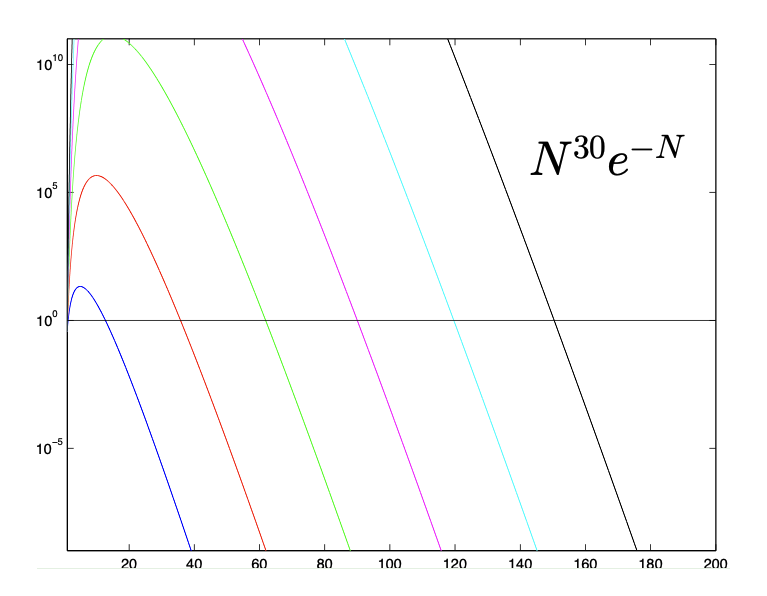
\includegraphics[width=0.5\textwidth]{img/vc-plot.png}
    \caption{The relationship between the probability of deviation and the number of samples, illustrating how the VC-dimension affects the generalisation bound. A higher VC-dimension or fewer samples increase the probability bound, indicating a lower confidence in generalisation.}
    \label{fig:vc_dimension_plot}
\end{figure}

The graph above shows how the bound on the generalisation error decreases with the number of samples $N$, for different values of the VC-dimension. It emphasises the trade-off between the complexity of the hypothesis class (as measured by the VC-dimension) and the amount of data required to ensure good generalisation with high probability.\\

\textbf{Rule of Thumb:}
A common heuristic is that the number of training examples $n$ should be at least an order of magnitude greater than the VC-dimension, i.e., $n \geq 10d_{VC}(\mathcal{H})$, to provide reasonable confidence in the generalisation of the learned hypothesis.


\subsection{Generalisation Error in the Context of the VC Inequality}

The VC Inequality provides a bound on the generalisation error for machine learning models. It establishes that with a high probability, the true risk \(R(h)\) for any hypothesis \(h\) from the hypothesis class \(\mathcal{H}\) will not be much higher than the empirical risk \(\widehat{R}_n(h)\), up to a complexity term that depends on the VC dimension of the hypothesis class.

\begin{definitionbox}{VC Inequality Error}\label{vc_inequality_error}
\[P\left(\sup_{h\in\mathcal{H}}|\widehat{R}_{n}(h)-R(h)|>\varepsilon\right)\leqslant4\underbrace{m_{\mathcal{H}}(2n)}_{\leqslant(2n+1)^{d_{VC}(\mathcal{H})}}e^{-\varepsilon^{2}n/8}\]
From the VC Inequality, we get a term for error on the rightmost square root term:

\[
R(h) \leq \widehat{R}_n(h) + \sqrt{\frac{8d_{VC}(\mathcal{H})}{n} \log\left(\frac{2n + 1}{\delta}\right) + \frac{8}{n} \log\frac{4}{\delta}}
\]

This error is called a complexity term, denoted as a function of $\Omega$ where:
\[
\Omega(n, \mathcal{H}, \delta ) = \sqrt{\frac{8d_{VC}(\mathcal{H})}{n} \log\left(\frac{2n + 1}{\delta}\right) + \frac{8}{n} \log\frac{4}{\delta}}
\]
\end{definitionbox}

This bound indicates that as the number of samples \(n\) increases, the gap between empirical risk and true risk closes, provided the VC dimension \(d_{VC}\) remains fixed.

\subsection{Performance vs. Complexity}

The graph below illustrates the trade-off between a model's complexity and its performance. The complexity is represented by the VC dimension, and the error is depicted on the vertical axis. 

\begin{figure}[H]
\centering
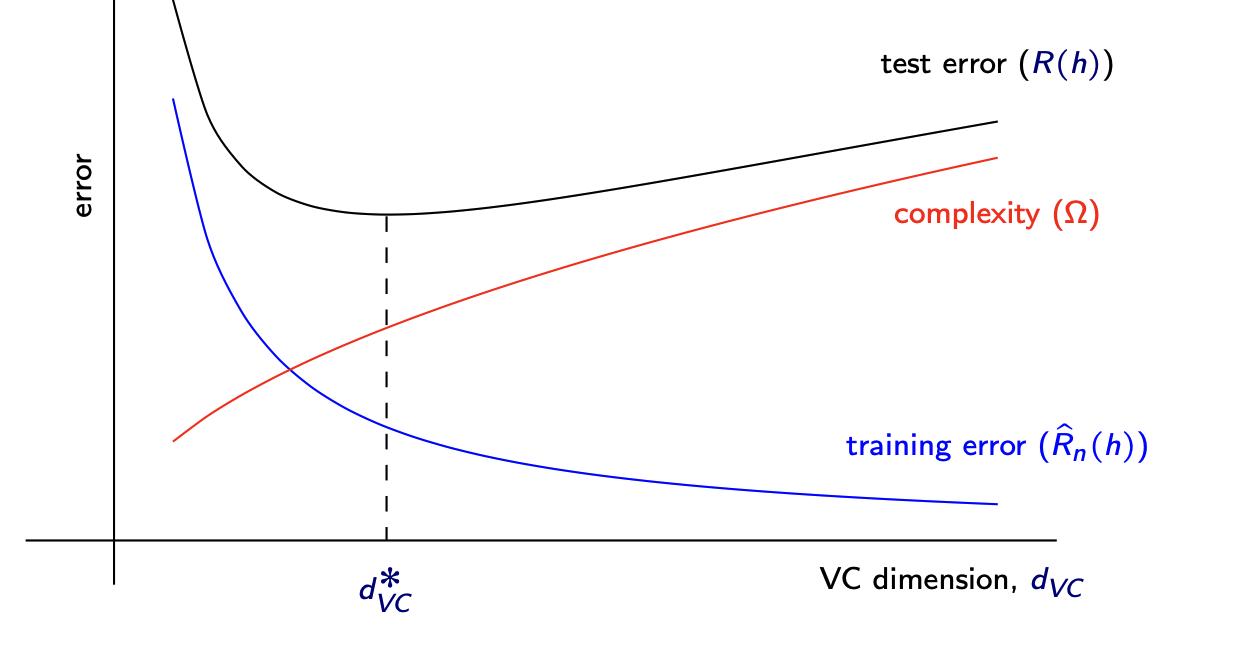
\includegraphics[width=0.8\textwidth]{img/perf-vs-cmplxty.png} % path to your image file
\caption{The trade-off between model complexity and performance. The blue curve represents the training error which decreases with model complexity, while the red curve represents the test error which initially decreases and then increases due to overfitting. The point where the test error is minimum corresponds to the optimal model complexity.}
\label{fig:performance_vs_complexity}
\end{figure}

As the VC dimension increases, the training error typically decreases as the model becomes more capable of fitting the training data. However, beyond a certain point, an increase in complexity leads to overfitting, and the test error begins to increase. The optimal VC dimension, \(d_{VC}^*\), is the point at which the test error is minimised, striking a balance between underfitting and overfitting.


\subsection{Polynomial Bounds on the Growth Function}

The growth function, denoted as \(m_{\mathcal{H}}(n)\), describes the maximum number of distinct outputs (or dichotomies) that a hypothesis class \(\mathcal{H}\) can produce for any sample of size \(n\). Understanding the behaviour of this function is key for assessing the capacity of the hypothesis class to fit various datasets.

Polynomial bounds on the growth function provide a way to approximate the complexity term \(\Omega(n, \mathcal{H}, \delta)\) in generalisation error bounds. Specifically:

\begin{itemize}
  \item The growth function \(m_{\mathcal{H}}(k)\) is bounded by a polynomial in \(n\), with the VC dimension acting as a break point. This means that for any sample size \(n\), the growth function \(m_{\mathcal{H}}(n)\) is at most polynomial in \(n\), which is significant as it limits the number of dichotomies the hypothesis class can shatter.
  
  \item When \(n\) is less than the VC dimension \(d_{VC}\), \(m_{\mathcal{H}}(n)\) can grow as fast as \(2^n\). However, once \(n\) exceeds \(d_{VC}\), the growth of \(m_{\mathcal{H}}(n)\) is significantly constrained, reflecting the limitations imposed by the finite VC dimension.
  
  \item A common polynomial bound is given by \(m_{\mathcal{H}}(n) \leq n^{d_{VC}} + 1\), which simplifies the expression and is more convenient to use than the exact polynomial form involving coefficients.
  
  \item For sufficiently large \(n\), an even tighter bound is often used:
  \[
  m_{\mathcal{H}}(n) \leq \left(\frac{ne}{d_{VC}}\right)^{d_{VC}}
  \] 
  where \(e\) is the base of the natural logarithm. This bound is known to be a more accurate estimate for the growth function when the sample size is large relative to the VC dimension (note that it is in a very similar form to the derivation in \ref{combquant_function_bound}).
\end{itemize}

These polynomial bounds are instrumental in deriving generalisation bounds such as those presented by the VC inequality, which connects the empirical risk with the true risk of a hypothesis.

\begin{examplebox}{Example Learning Question}
    In a binary classification problem, the test error is 27\% on 100 random test samples. Give a confidence interval that contains the expected test error with 90\% probability? How does the result change if the test error is obtained on 1000 samples? Use Hoeffding, and then VC assuming VC dimension of the hypothesis class is 3.\\

Let $X_i \in \{0,1\}$ denote the error in classifying sample $i$, $n$ the number of samples (100 or 1000), $\mu = \mathbb{E}[X_i]$ the expected test error, and $\nu = \frac{1}{n}\sum_{i=1}^{n} X_i = 0.27$ the empirical test error.\\

By Hoeffding's inequality,
\[ P(|\nu - \mu| \geq \epsilon) \leq 2e^{-2n\epsilon^2}. \]\\

Therefore, $\mu \in [\nu - \epsilon, \nu + \epsilon]$ with probability at least $1 - \delta = 1 - 2e^{-2n\epsilon^2}$. Setting $1 - \delta = 0.9$ and solving for $\epsilon$ we get $\epsilon = \sqrt{\log(2/\delta)/(2n)}$, which gives $\epsilon \approx 0.12$ for $n = 100$ and $\epsilon \approx 0.04$ for $n = 1000$. The required confidence intervals are approximately $[0.15, 0.39]$ for $n = 100$ and $[0.23, 0.31]$ for $n = 1000$.\\

Repeat with Vapnik-Chervonenkis Inequality:
\[ P(|\nu - \mu| \geq \epsilon) \leq 4(2n + 1)^{d_{VC}}e^{-\frac{n\epsilon^2}{8}}. \]\\

Given $\nu = 0.27$ and $d_{VC} = 3$, we want to solve for $\epsilon$.\\

We start by rearranging the inequality to solve for $\epsilon^2$:
\[ \epsilon^2 = \frac{8}{n} \log\left(\frac{4(2n + 1)^{d_{VC}}}{\delta}\right). \]\\

Substituting $d_{VC} = 3$ and for $n = 100$ and $1000$ samples, we can compute the specific values of $\epsilon$. 

\end{examplebox}

\begin{examplebox}{Inequality Bounds Question}
Given VC inequality \( P\left( \sup_{h\in\mathcal{H}} |\widehat{R}_n(h) - R(h)| > \epsilon \right) \leq 4m_{\mathcal{H}}(2n)e^{-\frac{n\epsilon^2}{8}} \), show how to arrive at the following generalisation bounds \( R(h) \leq \widehat{R}_n(h) + \Omega(n, \mathcal{H}, \delta) \):

\begin{itemize}
    \item[(a)] \(\Omega(n, \mathcal{H}, \delta) = \sqrt{\frac{8d_{VC}}{n} \log(2n + 1) + \frac{8}{n} \log \frac{4}{\delta}}\)
    \item[(b)] \(\Omega(n, \mathcal{H}, \delta) = \sqrt{\frac{8d_{VC}}{n} \log \frac{2ne}{d_{VC}} + \frac{8}{n} \log \frac{4}{\delta}}\)
    \item[(c)] \(\Omega(n, \mathcal{H}, \delta) = \sqrt{\frac{8d_{VC}}{n} \log 2n + \frac{8}{n} \log \frac{4}{\delta}}\)
\end{itemize}

From the slide on polynomial bounds we can use the following bounds in \( 4m_{\mathcal{H}}(2n)e^{-\frac{n\epsilon^2}{8}} \):
\begin{itemize}
    \item \( m_{\mathcal{H}}(n) = n^{d_{VC}} \)
    \item \( m_{\mathcal{H}}(n) = n^{d_{VC}} + 1 \)
    \item \( m_{\mathcal{H}}(n) = (n + 1)^{d_{VC}} \)
    \item \( m_{\mathcal{H}}(n) = \left(\frac{ne}{d_{VC}}\right)^{d_{VC}} \)
\end{itemize}

Plugging each of these into the VC inequality and solving for \( \epsilon \) gives us the various forms of the generalisation bounds.

\end{examplebox}

\begin{examplebox}{Combining Error Bounds Question}
    
Show how to arrive at the following expression:
Let \( g = \arg\min_{h\in\mathcal{H}} \widehat{R}_n(h) \) and \( h^* = \arg\min_{h\in\mathcal{H}} R(h) \). Then with probability at least \( 1 - \delta_1 - \delta_2 \),
\[
R(g) \leq R(h^*) + \sqrt{\frac{8d_{VC}(\mathcal{H})}{n} \log(2n + 1) + \frac{8}{n} \log \frac{4}{\delta_1} } + \sqrt{\frac{1}{2n} \log \frac{2}{\delta_2}}
\]

Hint: Use \( R(g) \), \( R(h^*) \), \( \widehat{R}_n(g) \), \( \widehat{R}_n(h^*) \),

\subsection*{Proof:}
We start by decomposing the difference between the true risk of \( g \) and the best possible hypothesis \( h^* \) as follows:
\[
R(g) - R(h^*) \leq \underbrace{|R(g) - \widehat{R}_n(g)|}_{\text{VC bound}} + \underbrace{|\widehat{R}_n(g) - \widehat{R}_n(h^*)|}_{\leq 0 \text{ by def. of g (ERM)}} + \underbrace{|\widehat{R}_n(h^*) - R(h^*)|}_{\text{Hoeffding Bound}}
\]
We use the VC bound for the first term, the definition of \( g \) ensures the second term is less than or equal to zero, and we use Hoeffding's bound for the last term. Combining these gives us our final result.

\end{examplebox}

\begin{examplebox}{Practical ML Scenario: Detecting Tax Evasion}
    The HMRC seeks to leverage machine learning (ML) to flag potential tax evasion in tax return submissions. The task is to construct an ML model that can distinguish between compliant and non-compliant cases with high confidence.\\

Given data:
\begin{itemize}
    \item Approximately 44,000 cases of tax evasion per year.
    \item 100 million tax returns submitted annually.
    \item Each tax return consists of 100 fields (features), structured and quantifiable.
    \item Historical data spans over the past 10 years.
\end{itemize}

\subsection*{Formulating the ML Problem}
\begin{itemize}
    \item We have a binary classification problem with labels $y \in \{-1,1\}$.
    \item The dataset consists of $n_p = 44000$ positive data points (indicative of tax evasion) and a total of $100M$ data points.
    \item To balance the dataset for learning, we will select a similar number of negative examples, giving us $n = 88000$ samples in total.
\end{itemize}

\subsection*{Defining the Error and Loss Function}
\begin{itemize}
    \item The error in classifying a sample $i$ is denoted by $X_i \in \{0,1\}$, where 1 represents an error (a case of tax evasion not detected or a false alarm).
    \item The empirical risk, or the average error over the dataset, is $\widehat{R}_n(h) = \frac{1}{n} \sum_{i=1}^{n} \mathbb{I}(h(x_i) \neq y_i)$.
    \item Given the high cost associated with false negatives (not detecting tax evasion), the loss function is heavily weighted towards such errors.
\end{itemize}

\subsection*{Choosing the Hypothesis Class}
\begin{itemize}
    \item We consider a hypothesis class $\mathcal{H}$ with a VC dimension $d_{VC} \leq 88000$, which could include polynomial classifiers of degree $k$ and linear classifiers.
    \item The Empirical Risk Minimization (ERM) strategy is employed to find the best hypothesis $g$ that minimizes the empirical risk.
\end{itemize}

\subsection*{Meeting HMRC's Performance Criteria}
\begin{itemize}
    \item The HMRC requires that the ML model's test error does not exceed the training error by more than 20\% with 99\% certainty.
    \item This requirement translates into selecting a hypothesis class $\mathcal{H}$ that satisfies the VC inequality for the given error rate $\epsilon = 0.2$ and confidence level $1 - \delta = 0.99$.
\end{itemize}

\subsection*{Applying the VC Inequality}
To calculate the bound on the VC dimension, we use the VC inequality:
\begin{equation*}
    P\left( |\widehat{R}_n(h) - R(h)| > \epsilon \right) \leq 4m_{\mathcal{H}}(2n)e^{-\frac{n\epsilon^2}{8}},
\end{equation*}
where $m_{\mathcal{H}}(n)$ represents the growth function of $\mathcal{H}$.

For $n = 88000$, $\epsilon = 0.2$, and $\delta = 0.01$, we solve for $d_{VC}$:
\begin{align*}
    0.01 & \geq 4 \cdot m_{\mathcal{H}}(2 \cdot 88000) \cdot e^{-\frac{88000 \cdot 0.2^2}{8}} \\
    0.01 & \approx 4 \cdot 88000^{d_{VC}} \cdot e^{-2.2 \cdot 88000} \\
    \log(0.01) & \geq d_{VC} \cdot \log(88000) - 2.2 \cdot 88000 \\
    d_{VC} & \leq \frac{\log(0.01) + 2.2 \cdot 88000}{\log(88000)}.
\end{align*}

After evaluating the above expression, we find that:
\begin{equation*}
    d_{VC} \leq 39.
\end{equation*}

Thus, we can conclude that the chosen hypothesis class should have a VC dimension of at most 39 to satisfy the HMRC's performance criteria.


\end{examplebox}

\section{Bias-Variance Tradeoff}
\subsection{Notation}
We now use $E_{out}$ to denote $R_n(g)$, the true/actual risk from the best hypothesis $g$ we picked that minimises empirical/testing risk. Conversely, $E_{in}$ denotes $\widehat{R}_n(g)$, the empirical risk for $g$. \\

\begin{commentbox}{Note to Self}
    Fix the notation to bold the vectors $x$, and the average hypothesis. `mathcal` the Ds as well.
\end{commentbox}



\subsection{Approximation-generalisation tradeoff}
We have covered VC analysis, which is: we can use another approach: bias-variance analysis. Before we get into this, let us recap:
\begin{itemize}
    \item We want to get small $R(g)$, or $E_{out}$, a low error in our out-of-sample testing. If it is small, then we have learned something. It shows we have a good approximation of target function $f$ out of sample.
    \item If we have a more complex hypothesis set $\mathcal{H}$, we have a better chance of \textbf{approximating} $f$ (our target function is more likely to be in the set), but with more complex, larger hypothesis set it will be difficult to choose the right hypothesis.
    \item Conversely, having a less complex $\mathcal{H}$ gives us a better chance of finding a good hypothesis that generalises out of sample.
    \item To find the best hypothesis which is the target function, we need to navigate the set – our only resource is the data we have to locate the best hypothesis. 
    \item The ideal hypothesis set $\mathcal{H}$ consists of just the target function $\{f\}$. Just like winning a lottery ticket. Although we will never get this in practice.




\end{itemize}
    From VC analysis, we can quantify the tradeoff as:
    \[E_{out} \leq E_{in} + \Omega\]
    \[R(g) \leq \widehat{R}_n(g) + \Omega\]

    \begin{definitionbox}{VC Inequality Error (from previous chapter)}
\[
R(h) \leq \widehat{R}_n(h) + \sqrt{\frac{8d_{VC}(\mathcal{H})}{n} \log\left(\frac{2n + 1}{\delta}\right) + \frac{8}{n} \log\frac{4}{\delta}}
\]
\end{definitionbox}


Bias-variance decomposes $E_{out}$ into a problem:
\begin{enumerate}
    \item How well can $\mathcal{H}$ approximate $f$?
    \item How well can we zoom in to select a good $h \in \mathcal{H}?$
\end{enumerate}

    
Our $E_{out}$ depends on the final hypothesis you pick.\\

We will take the difference between the error of the hypothesis chosen and the target function. The test error for a hypothesis \( g \) when tested on data set \( D \) is given by the expected value of the squared difference between the predicted value \( g^{(D)}(x) \) and the true function value \( f(x) \):
\begin{equation*}
R(g^{(D)}) = \mathbb{E}_x \left[ (g^{(D)}(x) - f(x))^2 \right]
\end{equation*}


The expected test error, considering many different training sets \( D_1, \dots, D_k \) and corresponding test sets \( (x_1, \dots, x_n)(D) \), is calculated as:
\begin{align*}
\mathbb{E} \left[ R(g^{(D)}) \right] &= \mathbb{E}_{D} \left[ \mathbb{E}_x \left[ (g^{(D)}(x) - f(x))^2 \right] \right] \\
&= \mathbb{E} \left[ (g^{(D)}(x) - f(x))^2 \right] \\
&= \mathbb{E}_x \left[ \mathbb{E}_{D} \left[ (g^{(D)}(x) - f(x))^2 \right] \right]
\end{align*}

Looking more closely at $\mathbb{E}_{D} \left[ \mathbb{E}_x \left[ (g^{(D)}(x) - f(x))^2 \right] \right]$, we define the `average hypothesis' $\bar{g}(x)=\mathbb{E}_{D}\left[g^{(D)}(x)\right]$. $x$ is fixed, so $g^{(D)}(x)$ is just a random variable, determined by your choice of data $D$.\\

Calculating the `average hypothesis' practically impossible since an expected value requires knowledge of the entire distribution. We could do a best estimation given \textbf{many} data sets $D_1, D_2, ... D_k$. Such an estimation is given by \[\frac1K\sum_{k=1}^{K}g^{(\mathcal{D}_{k})}(x)\]

Now, we have:

\[\begin{aligned}
\mathbb{E}_{\mathcal{D}}\left[(g^{(\mathcal{D})}(\mathbf{x})-f(\mathbf{x}))^2\right]& =\mathbb{E}_{\mathcal{D}}\left[(g^{(\mathcal{D})}(\mathbf{x})-\bar{g}(\mathbf{x})+\bar{g}(\mathbf{x})-f(\mathbf{x}))^2\right]  \\
&=\mathbb{E}_D\left[(g^{(\mathcal{D})}(\mathbf{x})-\bar{g}(\mathbf{x}))^2+(\bar{g}(\mathbf{x})-f(\mathbf{x}))^2\right. +\left.2(g^{(\mathcal{D})}(\mathbf{x})-\bar{g}(\mathbf{x}))(\bar{g}(\mathbf{x})-f(\mathbf{x}))\right] \\
&=\mathbb{E}_{\mathcal{D}}\left[(g^{(\mathcal{D})}(\mathbf{x})-\bar{g}(\mathbf{x}))^2\right]+(\bar{g}(\mathbf{x})-f(\mathbf{x}))^2 +2\underbrace{\mathbb{E}_{\mathcal{D}}\left[(g^{(\mathcal{D})}(\mathbf{x})-\bar{g}(\mathbf{x}))(\bar{g}(\mathbf{x})-f(\mathbf{x}))\right]}_{2(\bar{g}(\mathbf{x})-\bar{g}(\mathbf{x})) \text{is a constant}}\\
&= \underbrace{\mathbb{E}_{\mathcal{D}}\left[(g^{(\mathcal{D})}(\mathbf{x})-\bar{g}(\mathbf{x}))^2\right]}_{\mathrm{var}(\mathbf{x})}+\underbrace{(\bar{g}(\mathbf{x})-f(\mathbf{x}))^2}_{\mathrm{bias}(\mathbf{x})}.
\end{aligned}\]

Intuitively, we have:

\[\begin{aligned}
\mathbb{E}_{\mathcal{D}}\left[\left(\underbrace{g^{(\mathcal{D})}(\mathbf{x})}_{\text{some hypothesis}}-\underbrace{f(\mathbf{x})}_{\text{our target function}}\right)^2 \right]
&= \underbrace{\mathbb{E}_{\mathcal{D}}\left[\left(\overbrace{g^{(\mathcal{D})}(\mathbf{x})}^{\text{that hypothesis}}-\overbrace{\bar{g}(\mathbf{x})}^{\text{ best hypothesis from our data}}\right)^2\right]}_{\mathrm{var}(\mathbf{x})}\\
&+
\underbrace{\left( \overbrace{\bar{g}(\mathbf{x})}^{\text{ best hypothesis from our data}}-\overbrace{f(\mathbf{x})}^{\text{our target function}}\right)^2}_{\mathrm{bias}(\mathbf{x})}.
\end{aligned}\]


Taking this across many data sets D:
\[\begin{aligned}
\mathbb{E}\left[R(g^{(\mathcal{D})})\right]& =\mathbb{E}_{\mathcal{D}}\left[\mathbb{E}_{\mathbf{x}}\left[(g^{(\mathcal{D})}(\mathbf{x})-f(\mathbf{x}))^2\right]\right]  \\
&=\mathbb{E}_\mathbf{x}\left[\mathbb{E}_\mathcal{D}\left[(\mathbf{g}^{(\mathcal{D})}(\mathbf{x})-f(\mathbf{x}))^2\right]\right] \\
&=\mathbb{E}_\mathbf{x}\left[\text{bias}(\mathbf{x})+\text{var}(\mathbf{x})\right] \\
&=\text{bias}+\text{var}
\end{aligned}\]


\textbf{Bias} is the expected difference between the predictions of our model $\bar{g}(x)$ and the true function $f(x)$:
\begin{equation*}
\text{bias} = \mathbb{E}_x \left[ (\bar{g}(x) - f(x))^2 \right]
\end{equation*}
\begin{itemize}
    \item It measures how far $\bar{g}(x)$ is from $f(x)$.
    \item It is large if the hypothesis class $\mathcal{H}$ is small.
    \item It is small if $\mathcal{H}$ is large.
\end{itemize}

\textbf{Variance} is the expected value of the squared deviation of $g^{(D)}(x)$, a model trained on the dataset $D$, from the expected model $\bar{g}(x)$:
\begin{equation*}
\text{var} = \mathbb{E}_x \left[ \mathbb{E}_D \left[ (g^{(D)}(x) - \bar{g}(x))^2 \right] \right]
\end{equation*}
\begin{itemize}
    \item It quantifies how far $g^{(D)}(x)$ is from $\bar{g}(x)$.
    \item It is small if the hypothesis class $\mathcal{H}$ is small.
    \item It is large if $\mathcal{H}$ is large.
\end{itemize}

\begin{figure}[H]
    \centering
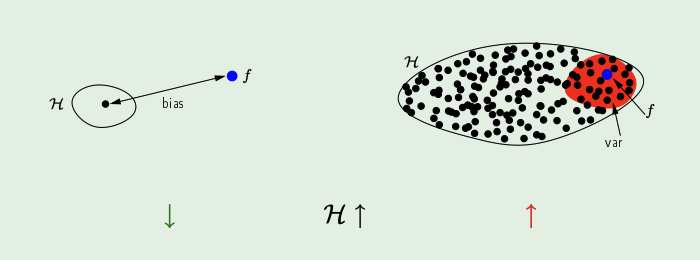
\includegraphics[width=0.75\textwidth]{img/bv.png}

    \caption{A visual description of bias and variance in varying hypothesis set sizes}
    \label{fig:bv-tradeoff}
\end{figure}

\subsection{Learning Curves}

For a simple model, the learning curve shows that as the number of data points increases, both the expected test error and the expected training error decrease, but there remains a gap between them due to model bias. The simple model may not be flexible enough to capture the underlying pattern in the data, resulting in higher bias.\\

In contrast, a complex model starts with a high expected test error which then rapidly decreases as more data points are added. The expected training error remains consistently low, even for small $n$, due to the model's high variance and low bias. However, without sufficient data, the complex model is at risk of overfitting, as indicated by the large gap between the training and test errors for smaller $n$.\\

The key is to find a model that balances the two, providing the best generalisation performance.


\begin{figure}[H]

    \centering
    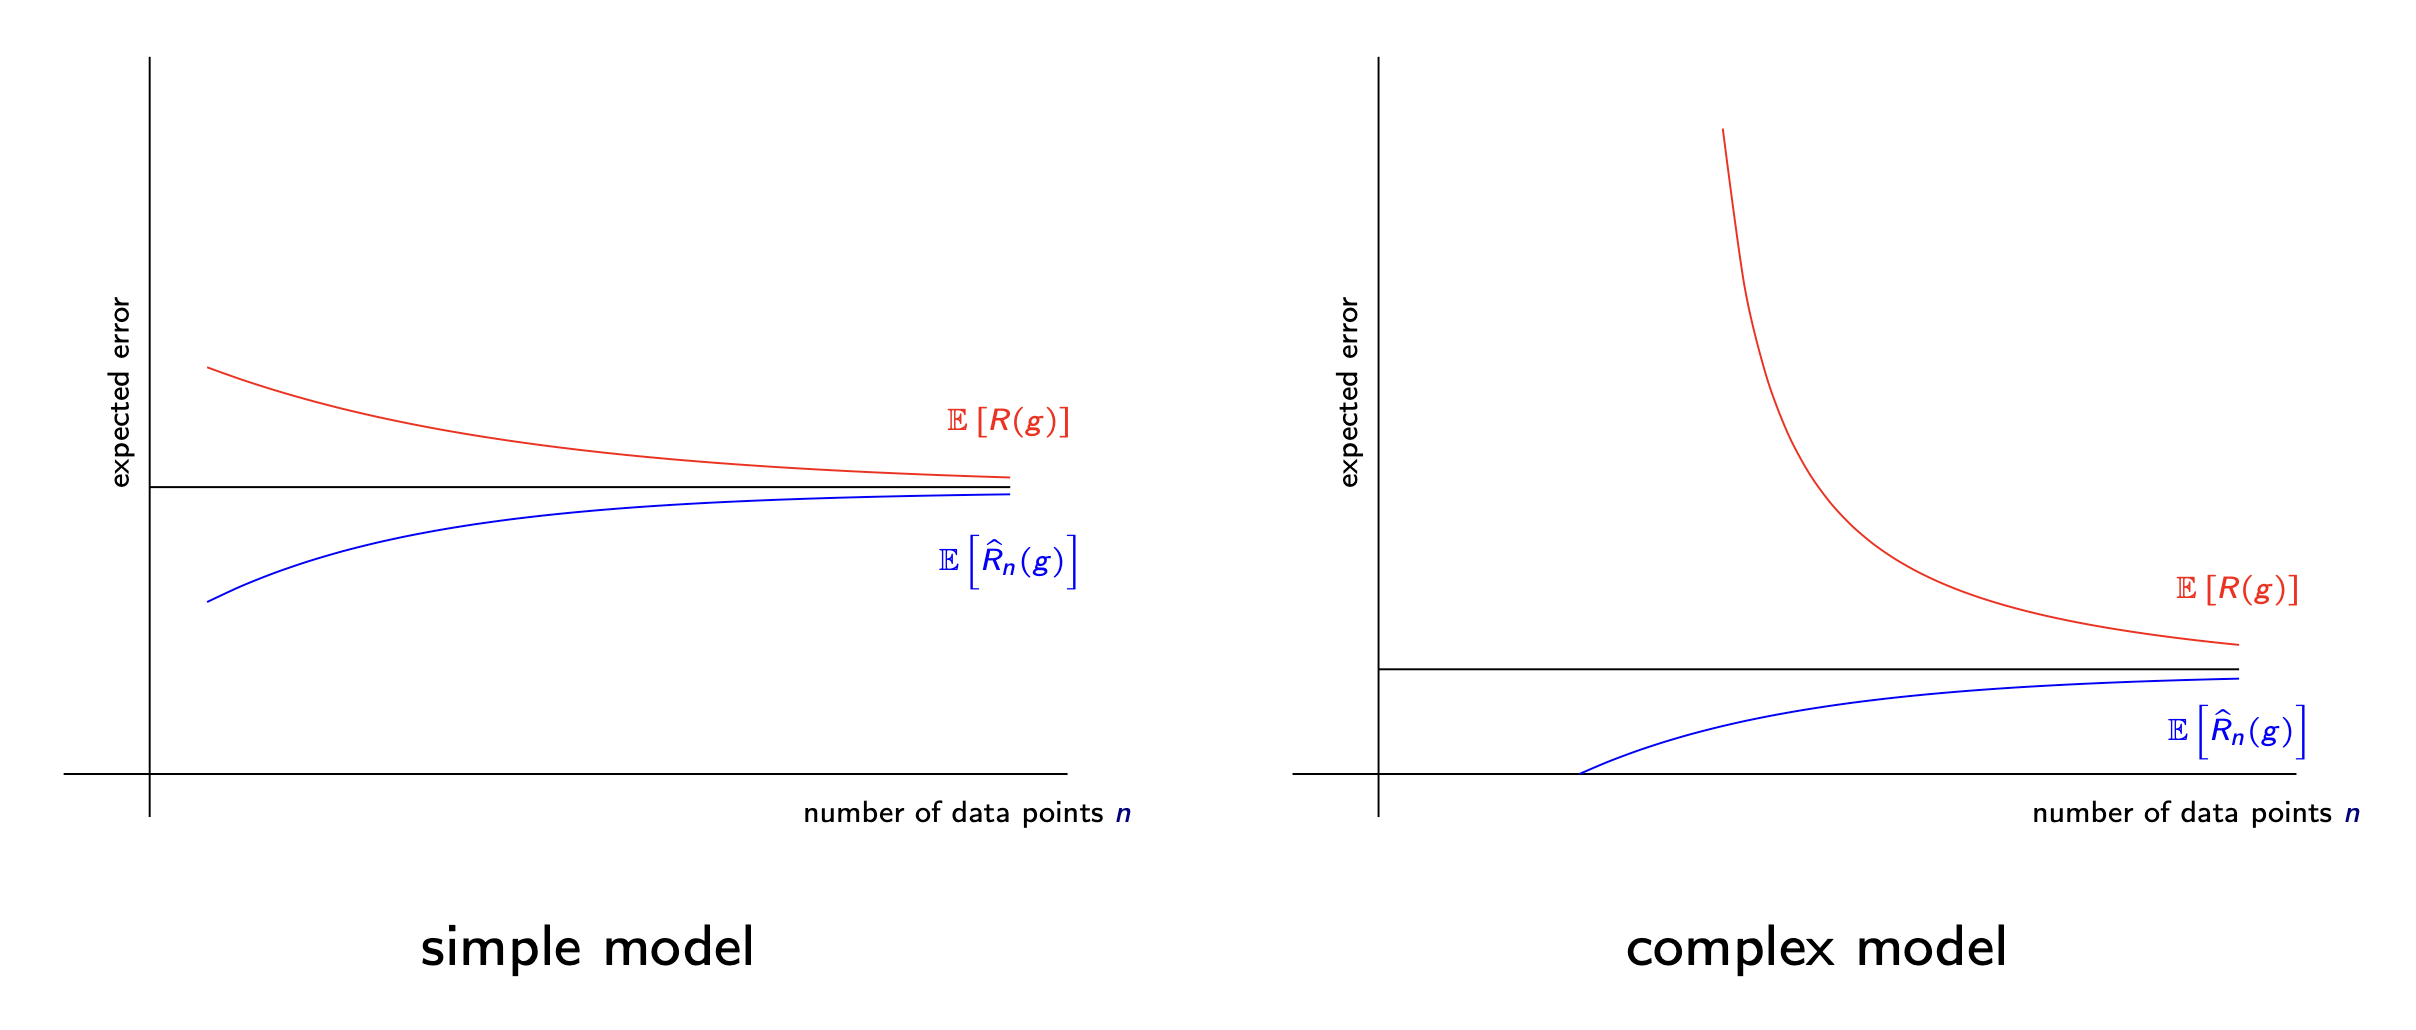
\includegraphics[width=1\linewidth]{img/learning_curves.png}
    \caption{The learning curves for simple (left) and complex (right) models showing the expected test error (red) and the expected training error (blue) as a function of the number of data points $n$.}
    
\end{figure}

\subsection{VC Analysis vs Bias Variance Analysis}
The VC analysis focuses on the relationship between the expected generalisation error and the size of the hypothesis class. It suggests that:
\begin{itemize}
    \item The best model approximation lies between the expected true error $\mathbb{E}[R(g)]$ and the expected empirical error $\mathbb{E}[\hat{R}_n(g)]$.
    \item In VC analysis, the error is estimated based on the training sample.
    \item The bias is determined by the best approximation $\bar{g}(x)$ (over all possible datasets $\mathcal{D}$).
    \item The bias is constant, depending solely on $\mathcal{H}$, and is independent of the number of data points $n$.
\end{itemize}

The bias-variance tradeoff, on the other hand, deals with the error due to bias and variance in the model:
\begin{itemize}
    \item Bias measures how far the average prediction $\bar{g}(x)$ is from the true function $f(x)$.
    \item Variance measures the fluctuation of $\bar{g}^{(\mathcal{D})}(x)$ around $\bar{g}(x)$ across different datasets $\mathcal{D}$.
    \item A small hypothesis class tends to have high bias and low variance, while a large hypothesis class tends to have low bias and high variance.
\end{itemize}

\begin{figure}[H]
    \centering
    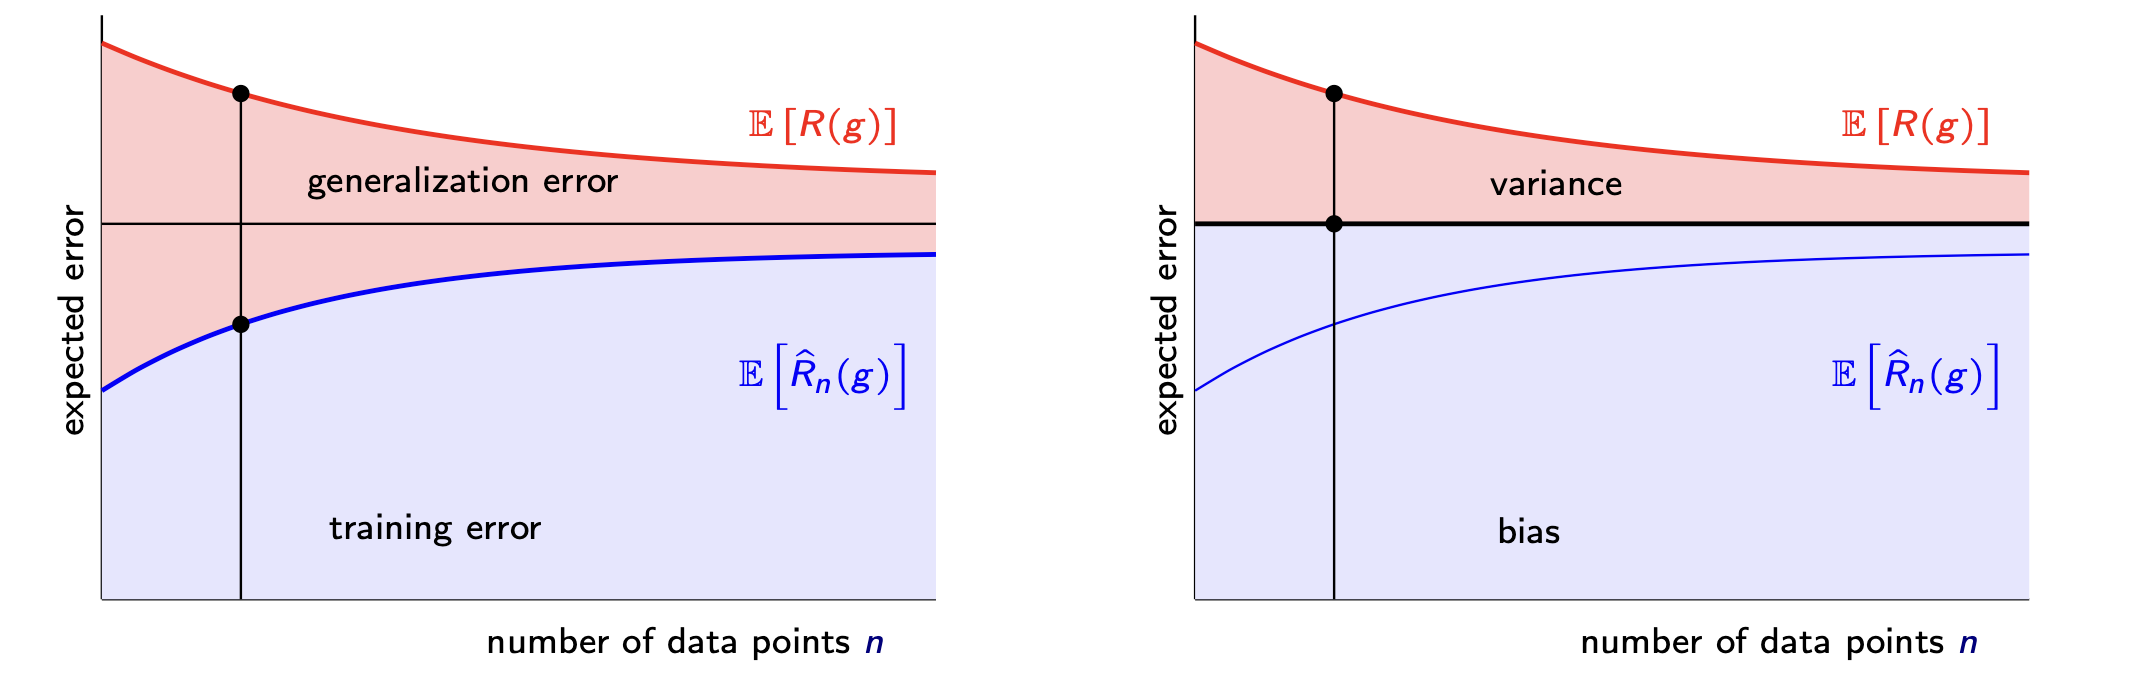
\includegraphics[width=1\linewidth]{img/vc_vs_bv.png}
    \caption{The left graph shows the generalisation error decreasing with the number of data points $n$ for a given hypothesis class $\mathcal{H}$. The right graph illustrates the bias-variance tradeoff, with the expected test error composed of both bias and variance components.}
    
\end{figure}

\section{Terminology}
\begin{commentbox}{Help from collaborators needed}
    Can someone help convert this slide into latex?
\begin{figure}[H]
    \centering
    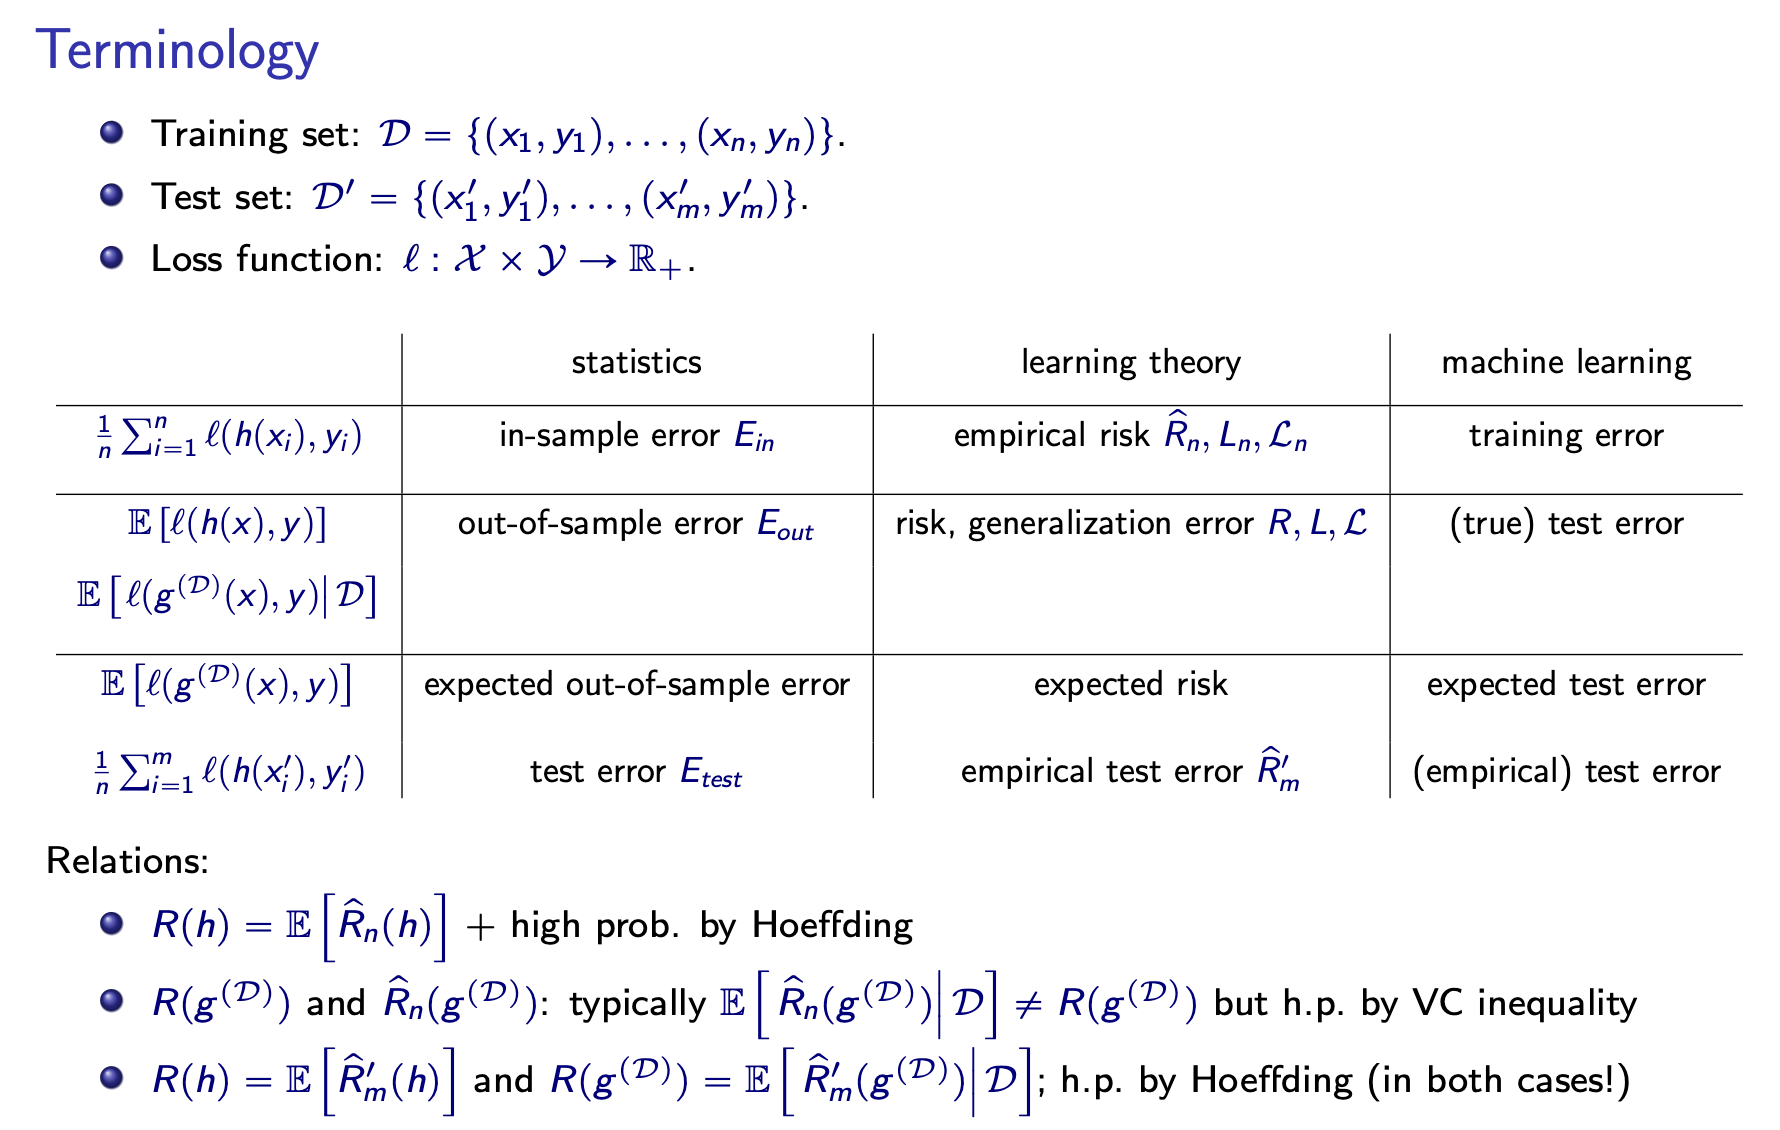
\includegraphics[width=1\linewidth]{img/2_terms.png}
\end{figure}
\end{commentbox}